%-----------------------------------------------------------------------------
\documentclass[12pt,a4paper]{report}
%---------------------------------------------------------------------------
\usepackage{amsmath}
\usepackage{amssymb}
\usepackage{amsthm}
% enumitem is loaded for the web build, not for the page layout. Without it
% tex4ht throws away the optional label on \item[(a).] and numbers the list
% 1, 2, 3 itself - so a question whose parts are (i), (ii), (iii) came out
% lettered a, b, c, and prose saying "the test in (a)" pointed at an item
% labelled "1.". With enumitem loaded the label survives verbatim, at every
% depth, and print and web finally agree.
\usepackage{enumitem}
\usepackage{amsfonts}
\usepackage{array}
\usepackage{longtable}
\usepackage{appendix}
\usepackage{blkarray}
\usepackage{bibentry}
\usepackage[none]{hyphenat}
\usepackage[noadjust]{cite}
\usepackage{filecontents}
\usepackage[all,knot,arc,poly]{xy}
\usepackage[pdftex]{graphicx}
\graphicspath{{images/}{../images/}}
\DeclareGraphicsExtensions{.pdf,.jpeg,.png, .jpg}
\usepackage{lscape}
\usepackage{epsfig}
\usepackage{mathrsfs}
\usepackage[left=40mm,right=25mm,top=25mm,bottom=25mm]{geometry}
\usepackage{url}
\usepackage{multicol}
\usepackage{multirow}
\usepackage{color}
\usepackage[table]{xcolor}
\definecolor{pink}{rgb}{1,0.5,0.5}
\usepackage{graphicx}
\graphicspath{ {images/} }
\usepackage{float}
\floatstyle{boxed} 
\restylefloat{figure}

\usepackage{tikz}
\usetikzlibrary{patterns,graphs,arrows.meta,shapes,trees,bending,fadings,quotes,angles}





\usepackage{pgfplots}
\usepgfplotslibrary{fillbetween}
\pgfplotsset{compat=1.18}

\usepackage{rotating}
%-----------------------------------------------------------------------------
\usepackage{setspace}
\usepackage{titletoc}
\titlecontents{chapter}
[0pt]
{\bfseries}
{\MakeUppercase\chaptername\ \thecontentslabel:\quad}
{\MakeUppercase}
{\hfill\contentspage}[]
%-----------------------------------------------------------------------------
\usepackage{float}
\textwidth 6.5in \textheight 9.175in\topmargin 0in \headheight 0in
\oddsidemargin 0in \evensidemargin 0in
\parskip 0.5\baselineskip
\parindent 0pt
\renewcommand{\baselinestretch}{1.25}
%-----------------------------------------------------------------------------
\theoremstyle{definition}
% One shared counter running chapter.section.n, as in the other courses here.
\newtheorem{thm}{Theorem}[section]
\newtheorem{defn}[thm]{Definition}
\newtheorem{exa}[thm]{Example}
\newtheorem{prop}[thm]{Proposition}
\newtheorem{coro}[thm]{Corollary}
\newtheorem{lem}[thm]{Lemma}
\newtheorem{result}[thm]{Result}
\newtheorem{exe}[thm]{Exercise}
\newtheorem*{note}{Note}
\newtheorem*{remark}{Remark}
\newtheorem{tech}{Technique}[section]
\newtheorem{fact}[thm]{Fact}
% A heading that is legal inside a theorem body, a list or a float, where
% \subsubsection is not.
\newcommand{\subhead}[1]{%
  \par\medskip\noindent\textbf{#1}\par\nobreak\smallskip}
\usepackage[nottoc]{tocbibind}
\renewcommand{\contentsname}{TABLE OF CONTENTS}
\renewcommand\bibname{REFERENCES}
%\renewcommand{\qedsymbol}{$\blacksquare$}

\parindent 0ex

%-----------------------------------------------------------------------------
\usepackage{titlesec}
\titleformat{\chapter}[hang]
          {\normalfont\filright\ttfamily\scshape\sffamily\bfseries
          	\centering\large}
          {\MakeUppercase{\chaptertitlename}\ \thechapter}{10pt\ :}{\large\MakeUppercase}        
          \titlespacing*{\chapter}{0pt}{-90pt}{16pt}
                       
\titleformat{\section}[hang]
           {\normalfont\sffamily\bfseries%
            \large}
            {\thesection.}{1ex}{}%[\titlerule]
%-----------------------------------------------------------------------------


%-----------------------------------------------------------------------------
\usepackage{fancyhdr}
\fancyhead{}

\pagestyle{fancy}

\fancyhf{}
%\fancyfoot[C]{\small Prepared by N.~Jeshurun \quad \thepage}

\fancyfoot[C]{\thepage}


%\fancyfoot[C]{\small Prepared by N.~Jeshurun}
\renewcommand{\headrulewidth}{0pt}
\renewcommand{\footrulewidth}{0pt}
%-----------------------------------------------------------------------------

\renewcommand{\sectionmark}[1]{\markright{}} %\thesection\ #1 (this one should be in th brackets, ayoub)
%-----------------------------------------------------------------------------

%-----------------------------------------------------------------------------


\newcommand{\bpf}{\noindent {\ttfamily  PROOF}. $\mbox{}$}
\newcommand{\epf}{\hfill \hbox{\raisebox{.5ex}{$\blacksquare$}$\phantom{.}$}}
%-----------------------------------------------------------------------------

% var, cov, bias and MSE are operator NAMES. Set as bare letters in maths they
% come out italic, so "var" reads as the product v.a.r -- the same defect as a
% bare \cos. These give them upright type and the correct spacing.
\DeclareMathOperator{\var}{var}
\DeclareMathOperator{\cov}{cov}
\DeclareMathOperator{\corr}{corr}
\DeclareMathOperator{\bias}{bias}
\DeclareMathOperator{\MSE}{MSE}

\newtheorem{problemx}{Problem}[section]
% The problem environment takes no source label. Marking a question
% "Test 2" or "2013 examination" turns it into something to be memorised
% rather than a topic to be understood, and it ties the question to one
% course's assessment when the same material is examined under several
% codes. Problems sit under the topic they belong to; that is the only
% label a reader needs.
\newenvironment{problem}{\begin{problemx}}{\end{problemx}}
\newenvironment{solution}
  {\renewcommand{\qedsymbol}{}\begin{proof}[\textit{Solution}.]}
  {\end{proof}}

% tex4ht expands amssymb's \checkmark in TEXT mode and hands MathJax the raw
% internals, so the reader sees \m@th \mathchar"458 instead of a tick.
% \ensuremath forces maths mode, where the token survives.
\let\amscheckmark\checkmark
\renewcommand{\checkmark}{\ensuremath{\amscheckmark}}

\begin{document}
% Title page depersonalised for the web, as with every other course here.
% The identity kept below is the Chapman-Kolmogorov equation, which is what the
% Markov property buys: the whole future is reachable one step at a time.
\begin{titlepage}
\thispagestyle{empty}
\begin{center}
\vspace*{3cm}
{\Huge\bfseries Stochastic Processes}\\[1.2cm]
{\large Lecture Notes}\\[2.5cm]
\line(1,0){300}\\[1.5cm]
$$p_{ij}^{(m+n)} = \sum_{k} p_{ik}^{(m)}\,p_{kj}^{(n)}$$
\end{center}
\end{titlepage}

\tableofcontents
\thispagestyle{empty}
\clearpage
\setcounter{page}{1}







\tableofcontents
\thispagestyle{empty}
\clearpage
\setcounter{page}{1}











\newpage
\chapter{Warming Up}




\section{Examples on Probability}
\begin{exa}
 When three fair dice are thrown, what will be the expected sum of numbers appearing.
\end{exa}


\begin{proof}[\textbf{\textit{Solution.}}]
Let $X_i$ denote the outcome on the $i^{\text{th}}$ dice
\begin{table}[H]
\centering
\begin{tabular}{cc}
$X_i$ & $P$\\
1    &  $1/6$\\
2    &  $1/6$\\
3   & $1/6$\\
4 & $1/6$\\
5 & $1/6$\\
6 & $1/6$\\
\end{tabular}
\hspace{1.5cm}
$E(X_i) = (1 + 2 + 3 + 4 + 5 + 6)\dfrac{1}{6} = \dfrac{7}{2}$
\end{table}

Let $X$ denote the sum of outcome of the dice. Hence
$$X  = X_1 + X_2 + X_3.$$
\begin{align*}
E(X) & = E(X_1) + E(X_2) + E(X_3)
      = 3\left(\frac{7}{2}\right) = \frac{21}{2}
      = 10.5.
\end{align*}
\end{proof}





\begin{exa}
At a party, $N$ men throw their hats into the centre of a room. The hats are mixed up and each man randomly selects one. Find the expected number of men who select their own hats.
\end{exa}



\begin{proof}[\textbf{\textit{Solution.}}]
Define a random variable $X_i$ as follows 

\[ X_i = 
\begin{cases}
1, \, & \text{if the }\hspace{0.2cm}i^{\text{th}}\hspace{0.2cm}\text{man picks his own hat}\\
0,  & \text{otherwise}\\
\end{cases}
\]

$ P(X_i = 1) = \dfrac{1}{N}\hspace{0.5cm}$ and $\hspace{0.5cm} P(X_i = 0) = \dfrac{N - 1}{N}\hspace{0.5cm}$ then we have that 
$E(X_i) = \dfrac{1}{N}.$\\

\text{Let}\hspace{0.5cm} $X  = X_1  + X_2 + \cdots\cdots + X_n$
\begin{align*}
E(X) & = E(X_1) + E(X_2) + \cdots\cdots + E(X_n)
      = N \times \dfrac{1}{N}
      = 1.
\end{align*}

Find $\, Var(X)$
\begin{align*}
Var(X) &  = Var(X_1 + X_2 + \cdots\cdots + X_n)
        = \sum_i Var(X_i) + 2\sum\sum_{i<j} Cov(X_i\, ,\, X_j).
\end{align*}
\begin{align*}
Var(X_i) & = \left(0 - \frac{1}{N}\right)^2 \times \frac{N - 1}{N} \, + \, \left(1 - \frac{1}{N}\right)^2\times \frac{1}{N}\\
         & = \frac{1}{N^2}\left(\frac{N - 1}{N}\right) \, + \, \left(1 - \frac{1}{N}\right)^2\cdot\frac{1}{N}\\
         & = \frac{1}{N}\left[\frac{N - 1}{N^2} + 1 + \frac{1}{N^2} - \frac{2}{N}\right]\\
         & = \frac{1}{N}\left[-\frac{1}{N} + 1\right]\\ 
         & = \frac{1}{N}\left(\frac{N - 1}{N}\right)\\
         & = \frac{N - 1}{N^2}.
\end{align*}
For $\, i < j$
\begin{align*}
Cov(X_i\, , \, X_j) & = E\left[\left(X_i - \frac{1}{N}\right)\left(X_j - \frac{1}{N}\right)\right]\\
& = E\left[X_iX_j - \frac{1}{N}\,X_i - \frac{1}{N}\, X_j + \frac{1}{N^2}\right]\\
& = E\left(X_iX_j\right) - \frac{1}{N}\cdot \frac{1}{N} - \frac{1}{N}\cdot\frac{1}{N} + \frac{1}{N^2}\\
& = E\left(X_iX_j\right) - \frac{1}{N^2}\\
& = 1\cdot P(X_i = 1\, , \, X_j = 1) - \frac{1}{N^2}\\
& = P\left( X_i = 1\big/ X_j = 1\right)\, P\left(X_j = 1\right) - \frac{1}{N^2}\\
& = \frac{1}{N - 1}\times \frac{1}{N} - \frac{1}{N^2}\\
& = \frac{1}{N(N - 1)} - \frac{1}{N^2}\\
& = \frac{N - (N - 1)}{N^2 (N - 1)}\\ 
& = \frac{N - N + 1}{N^2 (N - 1)}\\
& = \frac{1}{N^2 (N - 1)}.
\end{align*}
\begin{align*}
Var(X) & = \sum^N_{i = 1} Var(X_i) + 2\sum^{N-1}_{i<j}\sum^N Cov(X_i\, ,\, X_j)\\
 & = \sum^N_{i=1}\frac{N - 1}{N^2} + 2\sum^{N-1}_{i<j}\sum^N\frac{1}{N^2(N- 1)}\\
 & = 1.
\end{align*}
\end{proof}





\begin{exa}
Suppose there are 25 different of coupons and suppose that each time one obtains a coupon, it is equally likely to be any one of the 25 types.
Compute the expected number of different types that are contained in a set of 10 coupons.
\end{exa}



\begin{proof}[\textbf{\textit{Solution.}}]
Define a random variable $X_i$ such that 
\[X_i = 
\begin{cases}
0 & \text{if the}\hspace{0.2cm}i^{\text{th}}\hspace{0.2cm}\text{coupon is not there in the set of 10}\\
1 & \text{if atleast one}\hspace{0.2cm}i^{\text{th}}\hspace{0.2cm} \text{coupon is there in the set of 10}\\
\end{cases}
\]

$P(X_i = 0) = \left(\dfrac{24}{25}\right)^{10}$
\begin{align*}
P(X_i = 1) & = P(\text{atleast one}\hspace{0.2cm} i^{\text{th}}\hspace{0.2cm} \text{type is there in the set of 10})\\
& = 1  - P(X_i = 0)\\
& = 1 - \left(\dfrac{24}{25}\right)^{10}.
\end{align*}
$$E(X_i) = 1 - \left(\frac{24}{25}\right)^{10}.$$
Let $\, X = X_1  + X_2 + \cdots\cdots + X_{25}$
$$ E(X) = 25\left( 1 - \left(\frac{24}{25}\right)^{10}\right).$$
\end{proof}








\section{Conditional Expectation}
\begin{exa}
Let $X$ and $Y$ be independent Poisson random variables with respective means $\lambda_1$ and $\lambda_2$.
Find $P(X = r\big/ \, X + Y = n)$.
\end{exa}


\begin{proof}[\textbf{\textit{Solution.}}]
\begin{align*}
P(X = r\, \big/\, X + Y = n) & = \frac{P(X = r\, , \, X + Y = n)}{P(X + Y = n)}\\\\
& = \frac{P(X = r\, , \, Y = n - r)}{P(X + Y = n)}\\\\
& = \frac{P(X = r)\, P(Y = n - r)}{P(X + Y = n)}\\\\
& = \frac{\dfrac{e^{-\lambda_1} \, \lambda_1^r}{r!}\, \, \dfrac{e^{-\lambda_2}\, \, \lambda_2^{n-r}}{(n - r)!}}{\dfrac{e^{-(\lambda_1 + \lambda_2)}\, \, (\lambda_1 + \lambda_2)^n}{n!}}\\
& = C^n_r\, \, \frac{\lambda_1^r\, \lambda_2^{n - r}}{(\lambda_1 + \lambda_2)^n}\\
& = C^n_r\, \, \left(\frac{\lambda_1}{\lambda_1 + \lambda_2}\right)^r\,\, \left(\frac{\lambda_2}{\lambda_1 + \lambda_2}\right)^{n - r}\hspace{0.3cm} r = 0\, , \,  1\, , \, \cdots\cdots , \, n.
\end{align*}
\end{proof}











\section{Computing Expectations by Conditioning}
Let $X$ and $Y$ be discrete random variables 
$$E\left(X\big/\, Y = y\right) = \sum_x x\, P(X = x\, \big|\, Y = y)$$


What is $\, E(X/Y)$ ?
\begin{enumerate}
\item[] $E(X/Y)$ is a function of $Y$.
\item[] Also it is a random variable which assumes values like $E(X/Y= y)$ at $Y = y$.
\end{enumerate}

 
 
 
 
\begin{lem}
 Let $X$ and $Y$ be discrete random variables. Then $\, E\left( E\left(X/Y\right)\right) = E(X)$.
\end{lem}


\begin{proof}
\begin{align*}
E\left(E\left(X/Y\right)\right) & = \sum_y E\left(X/Y = y\right)\, P(Y  = y)\\
& = \sum_y\sum_x\, x\, P\left(X = x\, \big/\, Y = y\right)\, P(Y = y)\\
& = \sum_y \sum_x \, x\, P(X = x\, , \, Y = y)\\
& = \sum_x x\, \sum_y P(X = x\, ,  \, Y = y)\\
& = \sum_x x\, P(X = x)\\
& = E(X).
\end{align*}
\end{proof}





\begin{exa}
A miner is trapped in a mine containing three doors. The first door leads to a tunnel that takes him to safety after two hours of travel. The second door leads to a tunnel that returns him to the mine after three hours of travel. The third door leads to a tunnel that returns him to his mine after five hours.
Assuming that the miner is at all times equally likely to choose any one of the doors, what is the expected length of time until the miner reaches to safety.
\end{exa}


\begin{proof}[\textbf{\textit{Solution.}}]
$X:$ time to return to safety from mine.\\
Let $Y$ denote the door the miner chooses. $Y = y_i$ , if miner chooses $i^{\text{th}}$ door $(i = 1\, , \, 2\, , \, 3)$
\begin{align*}
E(X) & = E\left(E\left(X\big/Y\right)\right)\\
 & = \sum_y E(X/y = y)\, P(Y = y)\\
 & = 2\times \frac{1}{3} + \left(E(X) + 3\right)\times \frac{1}{3} + \left(E(X) + 5\right)\times\frac{1}{3}\\\\
 3\,E(X)  &  =  2 + E(X) + 3 + E(X) + 5
\end{align*}
$$E(X)  = 10\, hrs.$$
\end{proof}





 









\section{Computing Probability by Conditioning}
Let $E$ be an event. We will find $P(E)$. We define a random variable $X$ as follows
\[X = 
\begin{cases}
0 & \text{if}\hspace{0.2cm} E\hspace{0.2cm}\text{does not occur}\\
1 & \text{if}\hspace{0.2cm} E\hspace{0.2cm} \text{occurs}\\
\end{cases}
\] 

$$E(X) = 0\times P(E) + 1\times P(E) = P(E).$$



Let $Y$ be a discrete random variable. Then 
\begin{align*}
P(E) & = E(X) = E\left(E\left(X/Y\right)\right)
 = \sum_y E(X/Y = y)\, P(Y = y).\hspace{0.5cm}\cdots\cdots\hspace{0.5cm} (1)
\end{align*}
But 
\begin{align*}
E(X/Y = y) & = 0\times P(X = 0\, /\, Y = y) + 1\times P(X = 1\, /\, Y = y)\\
& = P(X = 1\, /\, Y = y)\\
& = P(E/Y=y).
\end{align*} 
Hence from $(1)$ we get $$P(E) = \sum_y P(E/Y = y)\, P(Y=y).$$
If $Y$ is continuous random variable, then $$P(E) = \int_{-\infty}^{\infty} P(E\, /\, Y = y)\, f_Y(y)\, dy.$$






\begin{exa}
An insurance company suppose that the number of accidents  that each of its policy holders will have in a  year is Poisson distributed, with the mean of the Poisson depending on the policy holder (age, gender etc).\\
If the Poison mean of a randomly chosen policy holder has a gamma distribution with density function.
$$g(\lambda) = \lambda \, e^{-\lambda}\hspace{0.3cm}, \hspace{0.3cm} \lambda \geq 0$$
What is the probability that a randomly chosen policy holder has a exactly $n$ accidents per year.
\end{exa}


\begin{proof}[\textbf{\textit{Solution.}}]
Let $X$ be the number of  accidents that a randomly chosen policy holder may have in a year.
\begin{align*}
P(X = n) & = \int^{\infty}_0P(X = n\, /\, \text{mean of}\hspace{0.2cm} X \hspace{0.2cm} \text{is}\hspace{0.2cm}\lambda)\, \lambda\, e^{-\lambda}\, d\lambda\\
& = \int_0^{\infty} \frac{e^{-\lambda}\, \lambda^n}{n!}\, \lambda\, e^{-\lambda}\, d\lambda\\
& = \frac{1}{n!}\int^{\infty}_0 e^{-2\lambda}\, \lambda^{n+1}\, d\lambda\hspace{1.5cm}\text{let}\hspace{0.5cm} \frac{m}{2} = \lambda\hspace{0.2cm}\implies \frac{dm}{2} = d\lambda\\
& = \frac{1}{n!}\int^{\infty}_0 e^{-m}\, \frac{m^{n + 1}}{2^{n + 1}}\, \frac{dm}{2}\\
& = \frac{1}{n!}\,\cdot\, \frac{1}{2^{n + 2}}\int_0^{\infty} e^{-m}\, m^{n + 1} \, dm\\
& = \frac{1}{n!}\cdot \frac{1}{2^{n + 2}}\, \Gamma(n + 2)\\
& = \frac{1}{n!}\cdot\frac{1}{2^{n + 2}}\, (n + 1)!\\
& = \frac{1}{n!}\cdot \frac{1}{2^{n + 2}}\cdot (n+1)\, n!\\
& = \frac{n + 1}{2^{n + 2}}.
\end{align*}
\end{proof}






\section{Markov's Inequality}
If $X$ is a random variable that takes only non-negative values, then for any $a>0$,
$$P\left(X \geq a\right) \leq \frac{E(X)}{a}.$$

\begin{proof}[\textbf{\textit{Proof.}}]
$\begin{aligned}[t]
E(X)  = \int_0^{\infty} x\, f(x)\, dx & = \int_0^ax\, f(x)\, dx \, + \, \int^{\infty}_ax\, f(x)\, dx\\
& \geq \int^{\infty}_a x\, f(x)\, dx\\
& \geq \int_a^{\infty}a\, f(x)\, dx\\
& = a\int^{\infty}_a f(x)\, dx\\
& = a\, P(X\geq a).
\end{aligned}$\\

Therefore $\, E(X) \geq a\, P(X\geq a)\hspace{0.3cm}\implies \, \dfrac{E(X)}{a}\geq P(X\geq a)$.
\end{proof}




\begin{exa}
Suppose  we know that the number of items produced in a  factory during a week is a random variable with mean 500.\\
What can be said about the probability that this week's production will be atleast 1000?
\end{exa}


\begin{proof}[\textbf{\textit{Solution.}}]
Let $X$ denote the weekly production.
$$P(X\geq 1000)  \leq \dfrac{E(X)}{1000}$$

$$\text{i.e}\hspace{0.3cm} P(X\geq 1000)  \leq \frac{500}{1000} = \frac{1}{2}.$$
\end{proof}







\section{Computing Variance by Conditioning}
$Var(X/Y)$ is a random variable. It's a function of $Y$.\\
When $Y = y,\hspace{0.3cm} Var(X/Y)$ assumes value $\, Var(X/Y = y)$.
\begin{align*}
Var(X/Y) & = E(X^2/Y = y) - \left( E(X/ Y = y)\right)^2\\
Var(X) & = E\left(Var(X/Y)\right) + Var\left(E(X/Y)\right)
\end{align*}




\begin{proof}[\textbf{\textit{Proof.}}]
$\begin{aligned}[t]
E\left(Var(X/Y)\right) & = E\left(E\left(X^2/Y\right)\right) - E\left(E(X/Y)\right)^2\\\\
& = E\left(X^2\right) - E\left(E(X/Y)\right)^2\hspace{0.5cm}\cdots\cdots\cdots\hspace{0.5cm} (1)
\end{aligned}$.
\begin{align*}
Var\left(E(X/Y)\right) & = E\left(\left(E(X/Y)\right)^2\right) - \left(E\left(E(X/Y)\right)\right)^2\\\\
& = E\left(\left(E\left(X/Y\right)\right)^2\right) - \left(E(X)\right)^2.
\end{align*}
$$E\left(\left(E(X/Y)\right)^2\right) = Var\left(E(X/Y)\right) + \left(E(X)\right)^2\hspace{0.5cm}\cdots\cdots\cdots\hspace{0.5cm}(2)$$
Substituting in (1) we get
$$E\left(Var(X/Y)\right) = E(X^2) - Var\left(E(X/Y)\right) - \left(E(X)\right)^2.$$
$$E\left(Var(X/Y)\right) + Var\left(E(X/Y)\right)  = E(X^2) - \left(E(X)\right)^2 = Var(X).$$
\end{proof}






\newpage
\chapter{Stochastic Process}

\section{Definitions}
Let $T$ be a subset of $\mathbb{R}$.\\
A collection of random variables $\{X(t)\, , \, t\in T\}$ is called  a stochastic process.\\

The index $t$ of $X(t)$ often represents time and describe the state of the process at time $t$ by random variable $X(t)$.\\

The set $T$ is called the \underline{index set} of the stochastic process $\{X(t)\, , \, t\in T\}$.\\

If $T$ is a countable set, the stochastic process is said to be disjoint time process.\\

If $T$ is an interval of real time, the stochastic process $\{X(t)\}$ is said to be a  continuous time process.\\

The set of all possible values that the random variable of the stochastic process $\{X(t)\, , \, t\in T\}$ can assume, is called the state space of the process.\\

The state space of a stochastic process can be discrete set or a continuous set.\\











\begin{exa}
\begin{enumerate}
\item Consider a computer server with jobs arriving at random points in time by customer and queuing for service. A customer departs from the system after service completion (all his jobs completed).\\
Let $N_k$ be the number of jobs in the system at the time of departures of  the $k^{\text{th}}$ customer.\\
Hence we have a  stochastic process $\{N_k\, , \, k = 1\, , \, 2\, \cdots\cdots \}$ whose state space $\, I = \{0\, , \,  1\, , 2\, \cdots\cdots\}$\\
(\textit{Discrete time and discrete state space}).

\item Let $X(t)$ be the number of jobs in the system at time $t$.\\
Hence we have a stochastic process $\{X(t)\, , \, t\geq 0\}\,$ where the state space $I= \{0\, , \, 1\, , \, 2\, \cdots\cdots\}$.

\item Let $W_k$ denote the time that the $k^{\text{th}}$ customer has to wait in the system before receiving service.\\
Hence we have a  stochastic process  $\{W_k\, , \, k = 1\, , \, 2\, , \cdots\cdots\, \}$ where $I = [0\, , \, \infty)$.

\item Let $Y(t)$ denote the cumulative service time required to complete all jobs in the system that are there at time $t$.\\
Hence we have a stochastic process $\{Y(t)\, , \, t\geq 0\}$ where state space $I= [0\, , \, \infty)$.
\end{enumerate}
\end{exa}








\section{Markovian Stochastic Process}
Consider a stochastic process $\, \{X(t)\, , \, t\in T\}\,$ which has a  countable state space.\\
The index set $T$ can be discrete or continuous. Hence we have the following two cases
\begin{enumerate}
\item $T$ is continuous.\\ Let $\, t_0 < t_1 < \, \cdots\cdots\, < t_n < t\, $ where $\, t_0\, , \, t_1\, \cdots\cdots\, t_n \in T$. Then the process $\{X(t)\}$ is Markovian if
$$P\left(X(t) = x\, |\, X(t_n) = x_n \, , \, x(t_{n - 1}) = x_{n - 1}\, , \cdots\cdots\, \,  X(t_0) = x_0\right) = P\left(X(t) = x\, |\, X(t_n) = x_n\right)$$
for all states $x$. 

\item $T$ is discrete.\\
Then the process $\, \{X_n\, , \, n = 0\, , \, 1\, , \, 2\, , \, \cdots\cdots\}$ is Markovian if 
$$P\left(X_{n + 1} = j\, |\, X_n = i_0\, ,\, X_{n - 1} = i_1\, , \, \cdots\cdots\,,\, X_0 = i_n\right) = P\left(X_{n + 1} = j\, |\, X_n = i_0\right)$$
for all states $j$.\\
\end{enumerate}







\section{Homogeneous Markov Processes}
\begin{enumerate}
\item $T$ is continuous.\\
Let $\, 0 < t_0 < t_n < t$. If 
$P\left(X(t) = j\, |\, X(t_n) = i\right)\, = \, P\left(X(t - t_n) = j\, |\, X(t_0) = i\right).$
Then the process $\{X(t)\}$ is a homogeneous Markov process.

\item $T$  is discrete. If 
$ P\left(X_{n + m} = j\, |\, X_m = i\right) \, = \, P\left(X_n = j\, |\, X_0 = i\right)$.
Then the Markovian process $\, \{X_n\, , \, n = 0\, , \, 1\, , \, 2\, , \, \cdots\cdots\}\,$ is homogeneous.\\
\end{enumerate}
\pagebreak






\newpage

\chapter{Markov  Chains}
A discrete time homogeneous Markov process is called a Markov chain.

\section{Introduction}
Consider a stochastic process $\{X_n , \, n = 0, \, 1, \, \cdots\}$. Let the statespace be $\, S = \{0, \, 1,\, \cdots\}$.\\

Assume $\, \{X_n\, , \, n = 0\, , \, 1\, , \, 2\, , \, \cdots\cdots\}$ is homogeneous Markov process. Then 
$$P\left(X_{n + 1} = j\, /\, X_n = i\right) \, = \, P\left(X_1 = j\, /\, X_0 = i\right)$$
Let $\, P\left(X_1 = j\, /\, X_0 = i\right)\, = \, P_{ij}$. We call $P_{ij}$ as one step transition probability from state $i$ to state $j$.\\

The probability satisfies the following:
\begin{enumerate}
\item[i).] $\, P_{ij}\geq 0\hspace{0.2cm} \forall\,  i \, \&\, j \, = 0\, , \, 1\, , \, 2\, , \, \cdots\cdots$
\item[ii).] $\displaystyle{\sum^{\infty}_{j = 0} P_{ij} = 1}$
\end{enumerate}


We arrange these one step transition probabilities in a matrix $P$ as follows:
$$ P = 
\begin{pmatrix}
P_{00} & P_{01} & P_{02} & \cdots\cdots\\
P_{10} & P_{11} & P_{12} & \cdots\cdots\\
P_{20} & P_{21} & P_{22} & \cdots\cdots\\
\vdots & \vdots & \vdots & \\
\end{pmatrix}$$
We note that every element in $P$ must be $\geq 0$ and also sum of elements of each row of $P$ is 1.\\






\begin{exa}
\begin{enumerate}
\item[a).] Weather conditions, rain or no rain previous day and not part weather conditions determines if it will rain next day or not.\\
Let $\alpha$ be the probability that if it rains today, then it will rain tomorrow. If it does not rain today, it will rain tomorrow with probability $\beta$. Describe this experiment as  a $\,\{X_n\, :\, n = 0\, , \, 1\, , \, 2\, , \, \cdots\cdots\}\,$ Markov chain.\\\\


Let random variable $X_n$ denote the weather of the $n^{\text{th}}$ day $\, \forall\, n  = 0\, , \, 1\, , \cdots$\\

$X_n$ can take only tow values Rain or not Rain

$$ P = 
\bordermatrix{~
 & \text{Rain} & \text{NotRain} \cr
\text{Rain} & \alpha & 1 - \alpha\cr
\text{NotRain} & \beta &  1 - \beta\cr}$$


\item[b).] Suppose that whether or not it rains today depends on previous weather conditions through the last two days. Specifically assume that if it has rained for the past two days, then it will rain tomorrow with probability 0.7; if it rained today but not yesterday then it will rain tomorrow with probability 0.5; if it rained yesterday but not today then it will rain tomorrow with probability 0.4; if it has not rained in the past two days then it will rain tomorrow with probability 0.2. Describe this experiment as a Markov chain.
$$ P = 
\bordermatrix{~
 & RR & R\overline{R}  & \overline{R}R & \overline{R}\, \overline{R}\cr
RR & .7 & .3 & 0 & 0\cr
R\overline{R} & 0 & 0 & .4 & .6\crcr
\overline{R}R & .5 & .5  & 0 & 0\cr
\overline{R}\, \overline{R} & 0 & 0 & .2 & .8\cr}$$

\item[c).] Balls are thrown one at a time and must land in one of the $k$ cells with equal probability. Let $X_n$ be the number  of occupied cells after the $n^{\text{th}}$ throw. Find the transition matrix for the chain $\,\{X_n\, :\, n = 0\, , \, 1\, , \, 2\, , \, \cdots\cdots\}\,$.

\item[d).] An Urn contains four balls, some are black, remaining are white. A ball is drawn at random. If it is black there is a probability $ 1- p$ that it will be returned to the urn, there is a probability $p$ that a white ball be returned to the urn instead. If it is white, it will be returned to the urn. This procedure is repeated indefinitely. Let $X_n$ be the number of black balls in the urn after the $n^{\text{th}}$ draw. Find the transition matrix for the chain $\,\{X_n\, :\, n = 0\, , \, 1\, , \, 2\, , \, \cdots\cdots\}\,$.


\item[e).] A company has three machines. Each day, independent of each other, a machine breaks down with probability $p$. Each night, there is one repair person who can repair only one machine. Let $X_n$ be the number of machines available at the beginning of the $n^{\text{th}}$ day. Find the transition matrix for the chain $\,\{X_n\, :\, n = 0\, , \, 1\, , \, 2\, , \, \cdots\cdots\}\,$.
\end{enumerate}
\end{exa}













\section{Chapman Kolmogrov Equations}
$n -$ Step transition probabilities
\begin{align*}
P_{ij}^n \, & = \, P\left(X_{n + m} = j\, \big/\, X_m = i\right)\hspace{0.5cm} \forall\, n > 0\, , \, \, \, i\,,\, \geq 0\\
& = P\left(X_n = j\, \big/\, X_0 = i\right).
\end{align*}






\textbf{Chapman Komogrov equations}\\
For any positive integers $n$ and $m$ and states $i$ and $j$,
$$P_{ij}^{n + m} \, = \, \sum_{k = 0}^{\infty}P_{ik}^m\, P_{kj}^n$$
\begin{proof}[\textbf{\textit{Proof.}}]
$\begin{aligned}[t]
P_{ij}^{n + m} \, & = \, P\left(X_{n + m} = j\, \big/\, X_0 = i\right)
 =  \sum_{k = 0}^{\infty} P\left(X_{n + m} = j\, , \, X_m = k\, \big/\, X_0  = i\right).
\end{aligned}$
\end{proof}







\section{Unconditional Distributions}
$$P_{ij}^n\left(X_n = j\, \big/\, X_0 = i\right)$$
Let $P_{(0)}$  be the initial distribution of Markov chain $\, \{X_n\, , \, n = 0\, , \, 1\, , \, 2\, , \, \cdots\cdots\cdots\}$ i.e we take $\, P_{(0)} = \left(\alpha_0\, , \, \alpha_1\, , \, \cdots\cdots\right)\,$ where $\, \alpha_i = P\left(X_0 = i\right)\hspace{0.3cm} \forall _i = 0\, , \, 1\, , \, 2\, , \, \cdots\cdots$\\

In general, we denote $P_{(n)}$ as the $n^{\text{th}}$ step unconditional distribution
\begin{align*}
P\left(X_1 = j\right)\, & = \sum^{\infty}_{i = 0} P\left(X_1 = j\, \big/\, X_0 = i\right)\, P\left(X_0 = i\right)\\
& = \, \sum^{\infty}_{i = 0} P_{ij}\, \alpha_i\\
& = \, \sum^{\infty}_{i = 0} \alpha_i\, P_{ij}\\
& = \, \text{this is the } \, (j)^{\text{th}}\, \text{element of }\, P_{(0)}P.
\end{align*}


Hence $\hspace{0.2cm} P_{(1)} = P_{(0)}P$
$$P_{(2)}  = P_{(1)}P = P_{(0)}PP = P_{(0)}P^2.$$
In general $\hspace{0.2cm} P_{(n)}\, = \, P_0\, P^n\hspace{0.2cm} \forall \, n = 1\, , \, 2\, , \, \cdots$\\


\begin{exa}
Suppose that  coin 1 has probability 0.7 of coming up heads and coin 2 has probability 0.6 of coming up heads.\\
If the coin flipped today comes up heads then we select coin 1  to flip tomorrow and if it comes up tails, then we select coin 2 to flip tomorrow.\\
If the coin initially flipped is equally likely to be coin 1 or coin 2 then what is the probability that  the coin flipped on the third day after the initial flip is coin 1?
\end{exa}


\begin{proof}[\textbf{\textit{Solution.}}]
$X_n \, = \, $ the coin flipped on the $n^{\text{th}}$  day\\

$S = \{$coin 1 $\, , \, $ coin 2$\}$
$$P = 
\bordermatrix{
 & C_1  & C_2\cr
C_1 & 0.7 & 0.3 \cr
C_2 & 0.6 & 0.4\cr}$$

\end{proof}


\begin{thm}[Path Analysis]
\begin{align*}
P\left(X_{n + 1} = j, \, X_n = i\, |\, X_{n - 1}  = k\right) & = P\left(X_{n + 1} = j/X_n = i,\, X_{n -1} = k\right)\, P\left(X_n = i/X_{n - 1} = k\right)\\
& = P\left(X_{n + 1} = j/X_n  = i\right)\, P\left(X_n = i/X_{n - 1} = k\right)\\
& = P_{ij}\, P_{ki}\\
& = P_{ki}\, P_{ij}.
\end{align*}
We note that $P^{(2)}_{kj}$ is the sum of probabilities of all routes from state $k$ to state $j$ in two steps.
\end{thm}







\begin{exa}
Consider a  Markov chain with the following transition matrix
$$\bordermatrix{~
   & A & B & C & D\cr
A & .1 & .3 & .2 & .4\cr
B & .2 & .3 & .2 & .3\cr
C & .3 & .3 & .1 & .3\cr
D & .2 & .1 & .4 & .3\cr}$$
Find $\, P\left(X_5 = A, \, X_4 =B, \, X_3 =C, \, X_2 = B, \, X_1 = A/ X_0 = B\right)$
\end{exa}


\begin{proof}[\textbf{\textit{Solution.}}]
 $$  = P_{BA}\, P_{AB}\, P_{BC}\, P_{CB}\, P_{BA} = (.2)(.3)(.2)(.3)(.2) = 0.00072.$$
\end{proof}
%-------------------------------------------



























\section{Classification of States}
\begin{defn}
\begin{enumerate}
\item[i.] State $j$ is said to be \textit{accessible} from state $i$ $(i\longrightarrow j)$ if $\exists$ a non negative integer $n$ such that $P^n_{ij} > 0.$
\item[ii.] States $i$ and $j$ \textit{communicate} if state $i$ is accessible from state $j$ and state $j$ is accessible from state $i$. In symbols we write $(i \longleftrightarrow j)$.
\end{enumerate}
\end{defn}


The relation of communication satisfies the following properties:
\begin{enumerate}
\item[(a)] State $i$ communicates with itself $i\longleftrightarrow i\hspace{0.2cm}\forall\hspace{0.1cm} $ states $i$.
\item[(b)]If state $i$ communicates with state $j$, then $j$ communicate with $i$.
\item[(c)] If state $i$ communicates with $j$ and state $j$ communicates with state $k$ then state $i$ communicates with state $k$ for any three states $i, j$ and $k$
\end{enumerate}



\begin{proof}
Since $\, i\longleftrightarrow j, \, \exists\, $ integers $m\geq 0$ such that $P^m_{ij} > 0$.\\
Similarly, $P^n_{jk} > 0$ for any integer $n\geq 0$
\begin{align*}
P_{ik}^{n + m} &  = \sum^{\infty}_{l = 0} P^m_{il}\, P^n_{lk} \hspace{0.3cm}(\text{Kolmogrov equation})\\
& > P^{m}_{ij}\, P^n_{ik}
\end{align*}
Hence $P^{n + m}_{ik} > 0$. Implying $i \longrightarrow k$.
Similarly we can show that $k\longrightarrow i$.\\
Combining $i \longrightarrow k, \hspace{0.2cm} k \longrightarrow i\, \implies \, i\longleftrightarrow k$.
\end{proof}


\begin{thm}[Partitioning of States into Classes]
Two states which communicate belong to the same classes.\vspace*{1pt}

If all the states of a Markov chain fall in one class, the chain is called \textit{irreducible}.
\end{thm}

\begin{proof}
Write $i \leftrightarrow j$ when $i$ and $j$ communicate, meaning
$p_{ij}^{(m)}>0$ and $p_{ji}^{(n)}>0$ for some $m,n$. The classes are the
equivalence classes of this relation, so it is enough to check it is an
equivalence relation.

\emph{Reflexive}: $p_{ii}^{(0)}=1$, so $i\leftrightarrow i$.
\emph{Symmetric}: immediate from the definition, which is symmetric in $i$ and
$j$.
\emph{Transitive}: suppose $i\leftrightarrow j$ and $j\leftrightarrow k$, with
$p_{ij}^{(m)}>0$ and $p_{jk}^{(n)}>0$. By the Chapman--Kolmogorov equation,
$$p_{ik}^{(m+n)} = \sum_{r} p_{ir}^{(m)}p_{rk}^{(n)} \geq p_{ij}^{(m)}p_{jk}^{(n)} > 0,$$
the inequality because every term of the sum is non-negative and $r=j$ is one of
them. The same argument in the other direction gives $p_{ki}^{(\cdot)}>0$, so
$i\leftrightarrow k$.

Hence communication partitions the state space, and two communicating states lie
in the same class.
\end{proof}

\begin{remark}
The one-line inequality $p_{ik}^{(m+n)}\geq p_{ij}^{(m)}p_{jk}^{(n)}$ is worth
keeping: it is Chapman--Kolmogorov used not as an identity but as a bound, by
retaining a single term of the sum, and most arguments about communication are
this inequality applied twice.
\end{remark}

\begin{exa}
Partition the states of Markov chain with the following transition matrix into classes
\begin{enumerate}
\item[(i)] $\bordermatrix{~
           & E_0  & E_1 & E_2\cr
      0   & \frac{1}{2} & \frac{1}{2}  & 0\cr
      1 & \frac{1}{2} & \frac{1}{4} & \frac{1}{4}\cr
      2 & 0 & \frac{1}{3} & \frac{2}{3}\cr}$\hspace{2cm}
      $\begin{matrix}
      E_0 \, \longleftrightarrow E_1\\
      E_1 \, \longleftrightarrow E_2\\
      E_0 \,\longleftrightarrow E_2\\
      E_0 \longrightarrow E_1 \longrightarrow E_2
      \end{matrix}$ The the chain is irreducible.
      
      
      
 \item[(ii).] $P = \bordermatrix{~
                & E_0 & E_1 & E_2 & E_3\cr
          E_0 & \frac{1}{2} & \frac{1}{2} & 0 & 0\cr
          E_1 & \frac{1}{2} & \frac{1}{2} & 0 & 0\cr
          E_2 & \frac{1}{4} & \frac{1}{4} & \frac{1}{4} & \frac{1}{4}\cr
          E_3 & 0  & 0 & 0 & 1\cr}$
          $$E_0 \longleftrightarrow E_1, \hspace{0.3cm} E_0\nrightarrow E_2, \hspace{0.3cm} E_1 \nrightarrow E_2$$
          
          $$C_1 = \{E_0, E_1\}\, , \hspace{0.4cm} C_2 = \{E_3\}\, , \hspace{0.4cm} C_3 = \{E_2\}.$$
\end{enumerate}
\end{exa}

A state is called \textit{absorbing} if at any step the chain is in that state then it remains there at all subsequent steps.\vspace*{0.6pt}

In this example state $E_3$ is an absorbing state.


\begin{thm}[Types of States]
Let $f_{ii}$ denote the probability that starting from state $i$, the chain will ever reenter state $i$.
\begin{enumerate}
\item[] If $f_{ii} = 1$, state $i$ is called recurrent.
\item[] If $f_{ii} < 1$, state $i$ is called transient.
\end{enumerate}
\end{thm}

\begin{proof}
Let $N$ be the number of returns to $i$, counting the visits after time zero.
Each time the chain is at $i$ it returns again with probability $f_{ii}$ and
never returns with probability $1-f_{ii}$, independently of the past by the
Markov property and time homogeneity. So $N$ is geometric:
$$P(N = n) = f_{ii}^{\,n}\left(1-f_{ii}\right),\qquad n=0,1,2,\dots$$

If $f_{ii}<1$ then $P(N=\infty)=0$ and $E(N) = f_{ii}/(1-f_{ii})<\infty$, so the
chain returns only finitely often: state $i$ is \emph{transient}. If
$f_{ii}=1$ then every trial succeeds, $N=\infty$ with probability one, and the
chain returns infinitely often: state $i$ is \emph{recurrent}.
\end{proof}

\begin{note}
Since $N$ counts returns, $E(N) = \sum_{n\geq1}p_{ii}^{(n)}$, so the dichotomy
can be read straight off the transition probabilities: $i$ is recurrent exactly
when $\sum_n p_{ii}^{(n)}$ diverges. That is the form used to settle the random
walks later in this chapter, where the sum is estimated rather than the return
probability computed directly.
\end{note}


\begin{exa}
Consider a Markov chain with the  following transition matrix
$$P =\bordermatrix{~
     & E_0 & E_1 & E_2 & E_3 & E_4  & E_5\cr
  E_0 & \frac{1}{2} & \frac{1}{2} &  0 & 0 & 0  &  0\cr
  E_1 & \frac{1}{2} & \frac{3}{4} & 0 & 0  & 0 & 0\cr
  E_2 & \frac{1}{4} & \frac{1}{4} & \frac{1}{4} & \frac{1}{4}  & 0 & 0\cr
  E_3 & \frac{1}{4} & 0 & \frac{1}{4} & \frac{1}{4} & 0 & \frac{1}{4}\cr
  E_4 & 0 & 0 & 0 & 0 & \frac{1}{2} & \frac{1}{2}\cr
  E_5 & 0  & 0 & 0 & 0 & \frac{1}{2} & \frac{1}{2}\cr}$$
Let $f_{ij}^{(n)}$ be the probability that chain visits state $j$  first time at steps $n$ given that it started from state $i$.\vspace*{1pt}

Computing $f_{11}$.\\

Clearly $\, f_{11} = \sum^{\infty}_{n = 1} f_{11}^n$
$$f^{(1)}_{11} = \frac{3}{4}$$
$f_{11}^{(2)}:\hspace{0.5cm} E_1\, \longrightarrow \, E_0\, \longrightarrow \, E_1$
$$f^{(2)}_{11} = \frac{1}{4}\cdot\frac{1}{2}$$
$f^{(3)}_{11}:\hspace{0.5cm} E_1 \longrightarrow \, E_0\, \longrightarrow \, E_0\, \longrightarrow\, \longrightarrow E_1$
$$f_{11}^{(3)}   = \frac{1}{4}\cdot\frac{1}{2}\cdot\frac{1}{2}$$
$f_{11}^{(4)}:\hspace{0.5cm} E_1 \longrightarrow \, E_0 \, \longrightarrow \, E_0 \longrightarrow E_0 \, \longrightarrow E_1$\\
$$f_{11}^{(4)}  = \dfrac{1}{4}\, \left(\dfrac{1}{2}\right)^{2}\, \dfrac{1}{2}$$

Therefore $$f^{(n)}_{11} = \frac{1}{4}\, \left(\frac{1}{2}\right)^{n - 2}\, \frac{1}{2}.$$
\begin{align*}
f_11 & = \frac{3}{4} + \frac{1}{8}\cdot\frac{1}{1 - \frac{1}{2}}\\
     & = \frac{3}{4}  + \frac{1}{4}\\
     & = 1.
\end{align*}

Hence state $E_1$ is recurrent. 
$$f_{11}^{(n)} , \, \hspace{0.4cm} n = 1, \, 2, \, \cdots\cdots$$
forms a probability function.\vspace*{10pt}

Mean Recurrence time of state $E_1$
\begin{align*}
\mu_1  &  = \sum^{\infty}_{n = 1}n\, f_{11}^{(n)}\\
       & = \frac{1}{8}\, \sum^{\infty}_{n = 1} n\, \left(\frac{1}{2}\right)^{n - 2}\\
       & = \frac{1}{2}\, \sum_{n =1}^{\infty} n\, \left(\frac{1}{2}\right)^n\\
       & = \frac{1}{4}\, \frac{1}{\left(1 - \frac{1}{2}\right)^2}\\
       &  = 1.
\end{align*}
\end{exa}









\begin{prop}
A state $i$ is recurrent if $\sum^{\infty}_{n = 1} P^n_{ii} = \infty.$
\end{prop}

\begin{proof}
Define a random variable $I_n$ as follows
\[ I_n = \begin{cases}
         1 & \text{if}\hspace{0.3cm} X_n  = i\\
         0 & \text{if} \hspace{0.3cm} X_n \neq i\\
          \end{cases}\]
Hence $\sum^{\infty}_{n = 0} I_n$ represents total visits to state $E_i$.
$$E\left[\sum^{\infty}_{n = 0} I_n \Big| X_0 = i\right] = \infty$$
if $E_1$ i recurrent.
\begin{align*}
E\left[\sum^{\infty}_{n = 0} I_n\, \Big|\, X_0 = i\right]  & = \sum^{\infty}_{n  = 0} \left[E(I_n /X_0  = i)\right]\\
 & = \sum^{\infty}_{n = 0} \left[1\times P(I_n  = 1\, / X_0 = 0) + 0\times P(I_n  = 0/X_0 = i)\right]\\
 & = \sum^{\infty}_{n  = 0} P(X_n   = i/ X_0 = i)\\
 & = \sum^{\infty}_{n = 0} P^n_{ii}
\end{align*}
But $E\left[\sum^{\infty}_{n = 0} I_n \, \Big|\, X_0 = i\right] = \infty $
$$\sum^{\infty}_{n = 0} P^n_{ii} = \infty.$$
\end{proof}





\begin{prop}
In a finite  states Markov chain not all states can be transient.
\end{prop}

\begin{proof}
Consider a Markov chain with State Space $\{0, \, 1, \, \cdots\, , \, m\}$. If possible assume all states are transient. Then the chain will visit State 0 in $T_0$ steps , 1 then transit into State 1 and remains there at $T_1$ steps and transit to $T_2$ and so hence after a finite number of steps no state will be visited which is a contradiction. Hence atleast one state is recurrent in a Markov chain which has finite number of states.
\end{proof}

\begin{coro}
If state $i$ is recurrent and State $i$  and $j$ communicate then State $j$ i is also recurrent.
\end{coro}

\begin{proof}
Since State $i$ is recurrent, $\sum_nP^n_{ii} = \infty$. Also $i\longleftrightarrow j$, therefore $\exists$ non negative integers $m$ and $k$ such that $$P^{m}_{ij} > 0\hspace{0.5cm} , \hspace{0.5cm} P^k_{ji} > 0$$
\begin{align*}
P^{k+n+m}_{jj}  & = \sum^{\infty}_{r =0} P^k_{ir}\, P^n_{rr}\, P^m_{rj}\\
& > P^k_{ji}\, P^n_{ii}\, P^m_{ij}
\end{align*}
Therefore
\begin{align*}
\sum_{n} P^{k + n + m}_{jj}  & > \sum_n P^k_{ji}\, P^n_{ii}\, P^m_{ij}\\
& = P^k_{ji}\, P^m_{ij}\, \sum_n P^n_{ii}\\
& = \infty.
\end{align*}
\end{proof}


Hence we conclude the following
\begin{enumerate}
\item[(i)] Recurrence is class property. i.e if  one State in a class is recurrent, then all other States in the same class will also be recurrent.
\end{enumerate}


In particular if one state in an irreducible Markov chain is recurrent, then all the States of the Markov chain will be recurrent.


\begin{exa}
Identify  the States of the Markov chain with the following transition matrix
$$\begin{pmatrix}
0 & 0 & \frac{1}{2} & \frac{1}{2}\\
1 & 0 & 0 & 0 \\
0 & 1 & 0 & 0\\
0 & 1 & 0 & 0\\
\end{pmatrix}$$
It is an irreducible chain.
\end{exa}



















\section{Random Walk Models}

\subsection{One Dimensional Random Walk}
Consider a Markov chain with States Space $\{0, \, \pm 1, \, \pm 2, \, \pm 3, \, \cdots\cdots \}$.\vspace*{1pt}

Suppose the transitions are done as follows
$$P_{i\, i+1}  = P$$
$$P_{i\, i -1} = 1 - P$$
This chain is called a \textit{one- dimensional random walk}.
$$P^{2n}_{00}  = \binom{2n}{n} \, P^n\, (1 - P)^{n}$$
Suppose that the chain is at $E_0$. After $2n$ transits, it can be in $E_0$ if number of transition in the right direction have to be equal to the number of transition in the left direction
$$P_{00}^{2n + 1}  = 0$$

$$P^{2n}_{00} = \frac{(2n)!}{n!\, n!} \, \left(P(1-P)\right)^n\, \hspace{0.2cm}  , \hspace{0.3cm} n = 1, \, 2, \, 3, \, \cdots\cdots$$

\textit{Sterling's approximation for $n!$}
$$n!\approx n^{n + \frac{1}{2}}\,  e^{-n}\, \sqrt{2\pi}.$$

Using Sterling's approximation for $n!$
\begin{align*}
P^{2n}_{00} & = \frac{(2n)^{2n + \frac{1}{2}}\, e^{-2n}\, \sqrt{2\pi}}{n^{n +\frac{1}{2}}\, e^{-n}\, \sqrt{2\pi}\, n^{n + \frac{1}{2}}\, e^{-n}\, \sqrt{2\pi}}\, \times\, \left(P(1 - P)\right)^n\\
& = \frac{1}{\sqrt{\pi}}\, 2^{2n}\, \cdot\, n^{2n + \frac{1}{2} - n - \frac{1}{2}  - n - \frac{1}{2}}\, \left(P(1 - P)\right)^n\\
 & = \frac{1}{\sqrt{\pi n}}\, 4^n\, \left(P(1 -P)\right)^n.
\end{align*}

$$\sum^{\infty}_{n = 1} P^{2n}_{00} = \sum^{\infty}_{n = 1} = \frac{1}{\sqrt{\pi n}}\, 4^n\, \left(P(1 -P)\right)^n.$$

\textbf{Case (i):} $\, P = \frac{1}{2}$
$$\sum^{\infty}_{n = 1} P^{2n}_{00} = \frac{1}{\sqrt{\pi}}\,\sum^{\infty}_{n = 1} \frac{1}{\sqrt{n}} = \infty$$ because $\sum_n\dfrac{1}{n^p}\, p-$ series is divergent for $0 < p < 1$.\vspace{2pt}

When $p = \frac{1}{2}$ all the States of one-dimensional random  walk are recurrent implying state $E_0$ is recurrent.\\


\textbf{Case (ii):} $p \neq \frac{1}{2}$\

Consider  $\, \hspace{0.3cm} 4P(1 - P) < 1$
$$4P -4P^2  < 1$$
$$1 + 4P^2 - 4P < 0$$
$$\text{i.e}\hspace{0.3cm} (2P - 1)^2 > 0$$
The inequality is true if $p\neq \frac{1}{2}$
$$\sum^{\infty}_{n = 1} P^{2n}_{00} = \sum_n \frac{1}{\sqrt{\pi n}}\, 4^n\, \left(P(1 - P)\right)^n  = \sum_n \frac{\left(4P(1 - P)\right)^n}{\sqrt{\pi n}}.$$
We'll apply ratio test to determine the convergence.
$$a_n = \frac{\left(4P(1 - P)\right)^n}{\sqrt{\pi n}}$$

$$a_{n +1} = \frac{\left(4P(1 - P)\right)^{n  + 1}}{\sqrt{\pi(n   + 1)}}$$

$$\frac{a_{n + 1}}{a_n} = \frac{\left(4P(1 - P)\right)}{\sqrt{1 + \frac{1}{n}}}$$ 

$$\lim_{n \rightarrow \infty} \frac{a_{n + 1}}{a_n} = 4P(1 - p) < 1.$$
Hence by ratio test
$$\sum_n P^{2n}_{00} < \infty$$
implying State $E_0$ is transient. Hence all states will be transient.





\subsection{Two Dimensional Symmetrical Random Walk}
At each transition, chain moves one step up or down or left or right, each with probability $\frac{1}{4}$. Hence the transition probabilities can be described as
$$P_{(i,j),(i + 1, j)}  = P_{(i,j),(i,j+1)} = P_{(i,j),(i-1,j)} =  P_{(i,j),(i,j-1)} = \frac{1}{4}, \hspace{0.3cm} i,j = 0,\, \pm 1,\, \pm 2, , \cdots$$
The Markov chain described by a two dimensional random variable is irreducible 
$$P^{2n}_{00} = \sum^n_{i =0} \frac{(2n)!}{i!\, i!\, (n -i)!\, (n - i)!} \, \left(\frac{1}{4}\right)^{2n}.$$

$$P^{2n + 1}_{00} = 0\hspace{0.6cm} \forall\, n = 1, \, 2,\, \cdots\cdots$$
\begin{align*}
P^{2n}_{00} = & \sum^n_{i = 0}\frac{(2n)!\, n!\, n!}{i!\, i!\, (n - i)!\, (n - i)!\, n!\, n!}\, \left(\frac{1}{4}\right)^{2n}\\
= & \sum^n_{i = 0} C_n^{2n}\, C_i^n\, C_i^n\, \left(\frac{1}{4}\right)^{2n}\\
 & \boxed{Note:\hspace{0.6cm}(x + y)^{2n} = (x + y)^n\cdot(x + y)^n\hspace{0.6cm}\text{and}\hspace{0.6cm} C^{2n}_n = \sum^n_{i = 0} C^n_i\, C^n_{n - i}}\\
 & = \left(\frac{1}{4}\right)^{2n}\, \binom{2n}{n}\, \sum_{i = 1}^n C^n_i\, C^n_{n - i}\\
 & = \left(\frac{1}{4}\right)^{2n}\, \binom{2n}{n}\, \binom{2n}{n}\\
 & \approx \sum_n \frac{1}{\pi\, n}. 
\end{align*}
Therefore
$$\sum^n_{i = 1} P^{2n}_{00} = \sum^{\infty}_{n = 1} \frac{1}{\pi\, n}$$ which diverges and hence $E_0$ is recurrent.



\subsection{Three Dimensional Symmetric Random Walk}
A particle moves in space, taking jumps of one unit in any one of the size directions $(\pm x, \pm y$ or $\pm z)$ with probability $\frac{1}{6}$.\\
We describe this walk as a Markov chain with infinite number of states.  We can argue as we did with one and two dimensional walks that the three dimensional random walk is also an irreducible Mark chain.\\
The State Space  $S = \{(i,j, k):\, i = 0, \pm 1, \, \pm 2, \cdots, \hspace{0.2cm} j = 0, \,  \pm 1, \, \pm 2, \, \cdots\, , \, \hspace{0.2cm} k =0, \, \pm 1, \, \pm 2, \, \cdots\}$\\
$P^{2n + 1}_{00} = 0\,$ for $n = 1, \, 2, \, \cdots\cdots$

\begin{align*}
P_{00}^{2n} & = \sum_{\substack{0\leq j + k \leq n\\ 0\leq j \leq n\\ 0\leq k \leq n}}\frac{(2n)!}{j!\, j!\, k!\, k!\, (n -j - k)! \, (n -j - k)!}\, \left(\frac{1}{6}\right)^{2n}\\
& = \left(\frac{1}{2}\right)^{2n}\, \binom{2n}{n}\, \sum_{0\leq j + k\leq n} \left(\frac{n!}{j!\, k!\, (n - j - k)!}\, \left(\frac{1}{3}\right)^n\right)^2
\end{align*}

Binomial Probability function $$ = \frac{n!}{j!\, (n - j)!} \, \left(\frac{1}{2}\right)^2.$$

Trinomial Probability function 
$$= \frac{n!}{j!\, k!\, (n - j - k)!}\, \left(\frac{1}{3}\right)^n = P$$
Then $\sum_{0\leq j + k \leq n} P = 1$
$$\sum_{0\leq  j + k \leq n} P^2 = \sum_{0\leq j + k \leq n} P\, P \leq \sum \max P\cdot P = \max P \sum P = \max P.$$
Thus
\begin{align*}
P^{2n}_{00} & = \left(\frac{1}{2}\right)^{2n}\, \binom{2n}{n}\, \sum P^2\\
& = \left(\frac{1}{2}\right)^{2n}\, \binom{2n}{n}\, \max P.
\end{align*}
Thus $P$ is maximum when $j = \frac{n}{3}, \hspace{0.2cm} k = \frac{k}{3}$
$$P^{2n}_{00} \leq \left(\frac{1}{2}\right)^{2n}\, \binom{2n}{n}\, \frac{n!}{\left(\frac{1}{3}\right)!\, \left(\frac{n}{3}\right)!\, \left(\frac{n}{3}\right)!}\, \left(\frac{1}{3}\right)^n.$$

Simplify and use Sterling's approximation for $n!$ and show that 
$$P^{2n}_{00} \leq \, \text{constant}\, \leq \frac{1}{n^{\frac{3}{2}}}$$
$$\sum P_{00}^{2n} \leq C \, \sum \frac{1}{n^{\frac{3}{2}}} < \infty.$$
Therefore $E_0$ is transient.




\section{Limiting probabilities}
\textit{Mean recurrent time:} starting  from state $E_i$, the expected steps chain takes to  return to state $E_i$.\vspace*{1pt}

For a recurrent state $\, f_{ii} = 1$. i.e $\left\{f^n_{ii} , \, n = 1, 2, \, \cdots\right\}$ forms a probability function. Hence mean recurrent time of a recurrent state $E_i$ is defined as 
$$\mu = \sum^{\infty}_{n = 1} n\, f_{ii}^n$$
$\mu$ can be a finite or infinite.\\
If $\mu < \infty$, then state $E_i$ is called \textit{positive recurrent}.\\
If $\mu = \infty$ , state $E_i$ is called \textit{null recurrent}.\vspace*{1pt}

In a finite states Markov chain, if a state is recurrent it will always be positive recurrent.\vspace{1pt}

\textit{Aperiodic State}. Let 
$$\begin{matrix}
P^n_{ii} & > 0, & n  = d, \, 2d, \, 3d, \, \cdots\\\\
         & = 0, & n  \neq d, \, 2d, \, 3d, \, \cdots
\end{matrix}$$
where $d$ is a positive integer $> 1$.
Then state $E_i$ is called periodic and the period is $d$.\vspace{1pt}

If $P^n_{ii} > 0$ for  $n = 1, \, 2, \, \cdots$ then state $E_i$ is called aperiodic. i.e there is positive probability of  a transition from $E_i$ to $E_i$ at every jump.


\begin{exa}
Consider a Markov chain with transition matrix
$$P = \bordermatrix{~
     & E_0 & E_1 & E_2 & E_3 & E_4\cr
E_0  & 0   & 0 & 0 & 0  & 1\cr
E_1 & 1 & 0 & 0 & 0 & 0\cr
E_2 & \frac{1}{2} & \frac{1}{2} & 0 & 0 & 0\cr
E_3 & \frac{1}{3} & \frac{1}{3} & \frac{1}{3} & 0 & 0\cr
E_4 & \frac{1}{4} & \frac{1}{4} & \frac{1}{4} & \frac{1}{4} & 0\cr}$$
\end{exa}

$P^{(2)}_{00} = P_{04}\, P_{4,0} \, > 0$\\
$P^{(3)}_{00} = P_{04}\, P_{41}\,P_{10} \, > 0$\\
$P^{(4)}_{00} = P_{04}\, P_{43}\, P_{32}\, P_{20}\, > 0$\\

$E_3$ is aperiodic.\\

A positive recurrent and aperiodic state is called \textit{ergodic state}.\\


\textbf{\bf \large{Limiting (stationary or equilibrium) distribution}}\\
Let $P = \begin{pmatrix}
          .4 & .1 & .5\\
          .2 & .2 & .6\\
          .3 & .4 & .3\\
         \end{pmatrix}\hspace{0.3cm}$ and $P_{(0)} = \begin{pmatrix}
                                                      .3 & .4 & .3\\
                                                     \end{pmatrix}$.
All the three states are egordic


\begin{table}[H]
\centering
\begin{tabular}{ccccc}
$n$ && $P^{(n)}$ && $P_{(n)}$\\\\
1 && $\begin{pmatrix}
       .4 & .1 & .5\\
       .2 & .2 & .6\\
       .3 & .4 & .3\\
      \end{pmatrix}$ && $\begin{pmatrix}
                          .29 & .23 & .48\\
                         \end{pmatrix}$\\\\
2 && $\begin{pmatrix}
        .33 & .26 & .41\\
        .3  & .3  & .4\\
        .29 & .23 & .48\\
      \end{pmatrix}$ && $\begin{pmatrix}
                           .306 & .267 & .427\\
                          \end{pmatrix}$\\
\vdots &&&&\\ \vdots &&&&\\
4 && $\begin{pmatrix}
        .3058 & .2581 & .4361\\
        .3050 & .2600 & .4350\\
        .3039 & .2548 & .4413\\
       \end{pmatrix}$ && $\begin{pmatrix}
                          .30481 & .25787 & .4322\\
                         \end{pmatrix}$\\\\
\vdots &&&&\\ \vdots &&&&\\
6 && $\begin{pmatrix}
       .3648 & .2572 & .4379\\
       .3048 & .2573 & .4378\\
       .30   & .2569 & .4383\\
     \end{pmatrix}$ && $\begin{pmatrix}
                        .30477 & .25720 & .43302\\
                       \end{pmatrix}$
\end{tabular}
\end{table}


We note that for large values of $n$, the rows of $P^{(n)}$ are equal and the unconditional distribution $P_{(n)}$ also does not change.\\


\textbf{\bf{Limiting distribution}}. Sequence of unconditional distribution $P_{(0)}, \, P_{(1)}, \, \cdots$ converges to some distribution $\pi$ of
\begin{enumerate}
\item[(i)] $\lim_{n\rightarrow \infty} P^n_{ij}\hspace{0.3cm}$ exist
\item[(ii)] $\lim_{n\rightarrow \infty} P^{(n)}_{ij}\hspace{0.2cm}$ is independent of $i$.
\end{enumerate}



\begin{thm}
For an irreducible ergodic Markov chain, $\lim_{n\rightarrow \infty} P^n_{ij}\,$ exist and is independent of $i$.\\

Let $\, \lim_{n\rightarrow\infty} P^{(n)}_{ij} = \pi_j\,\, , \hspace{0.3cm} j\geq 0$. Then $\pi_j$ is the unique solution of equation
$$\pi_j = \sum^{\infty}_{i = 0} \pi_i\, P_{ij}\, , \hspace{0.2cm} j\geq 0\hspace{0.3cm}\text{and}\hspace{0.3cm} \sum^{\infty}_{j  = 0} \pi_j = 1.$$
\end{thm}


\begin{exa}
Consider a Markov chain with states $\, 0, \, 1, \, 2, \, 3, \, 4.$\\ Suppose $P_{04} = 1$, and suppose that when the chain is in state $i, \, i>0$, the next state s equally likely to be any of the states $0,\, 1, \, \cdots\, , \, i - 1$. Find the limiting probabilities of this Markov chain
$$P = \bordermatrix{~
   & E_0 & E_1 & E_2 & E_3 & E_4\cr
E_0 & 0 & 0 & 0 & 0 & 1\cr
E_1 & 1 & 0 & 0 & 0 & 0\cr
E_2 & \frac{1}{2} & \frac{1}{2} & 0 & 0 & 0\cr
E_3 & \frac{1}{3} & \frac{1}{3} & \frac{1}{3} & 0 & 0\cr
E_4 & \frac{1}{4} & \frac{1}{4} & \frac{1}{4} & \frac{1}{4} & 0\cr}$$
\end{exa}

\begin{proof}[\textbf{\textit{Solution.}}]
Let $\pi = \begin{pmatrix}
            \pi_0, & \pi_1, & \pi_2, & \pi_3, & \pi_4\\
          \end{pmatrix}\,$ be the limiting distribution
          $$\pi = \pi\, P$$
          
          $$\begin{pmatrix}
            \pi_0, & \pi_1, & \pi_2, & \pi_3, & \pi_4\\
          \end{pmatrix} = \begin{pmatrix}
            \pi_0 & \pi_1 & \pi_2 & \pi_3 & \pi_4\\
          \end{pmatrix}\times
          \begin{pmatrix}
           0 & 0 & 0 & 0 & 1\\
           1 & 0 & 0 & 0 & 0\\
           \frac{1}{2} & \frac{1}{2} & 0 & 0 & 0\\
           \frac{1}{3} & \frac{1}{3} & \frac{1}{3} & 0 & 0\\
          \frac{1}{4} & \frac{1}{4} & \frac{1}{4} & \frac{1}{4} & 0\\
          \end{pmatrix}$$
          
 \begin{align*}
 \pi_0 & = \pi_1 + \frac{1}{2}\, \pi_2 + \frac{1}{3}\, \pi_3 + \frac{1}{4}\, \pi_4\\
 \pi_1 & = \frac{1}{2}\, \pi_2 + \frac{1}{3}\, \pi_3 + \frac{1}{4}\, \pi_4\\
 \pi_2 & = \frac{1}{3}\, \pi_3 + \frac{1}{4}\, \pi_4\\
 \pi_3 & = \frac{1}{4}\, \pi_4\\
 \pi_4 & = \pi_0
 \end{align*}
 Also $\hspace{0.3cm} \pi_0 + \pi_1 + \pi_2  + \pi_3 + \pi_4 = 1$
 \begin{align*}
 \pi_4 &  = \pi_0\\
 \pi_3  & = \frac{1}{4}\,\cdot\pi_0\\
 \pi_2 & = \frac{1}{3}\left(\frac{1}{4}\,\pi_0\right) + \frac{1}{4}\, \pi_0 = \frac{4}{12}\, \pi_0 = \frac{1}{3}\,\cdot\, \pi_0\\
 \pi_1 & = \frac{1}{2}\left(\frac{1}{3}\pi_0\right) + \frac{1}{3}\left(\frac{1}{4}\pi_0\right) + \frac{1}{4}\pi_0 = \frac{1}{2}\, \cdot\, \pi_0
 \end{align*}
 $$\pi_0 = \pi_0\left(\frac{1}{2} + \frac{1}{2}\cdot\frac{1}{3} + \frac{1}{3}\cdot\frac{1}{4} + \frac{1}{4}\right) = \pi_0\left(\frac{6 + 2 + 1 + 3}{12}\right)$$
 
 Since  $\hspace{0.3cm} \pi_0 + \pi_1 + \pi_2  + \pi_3 + \pi_4 = 1$. Hence
 $$\pi_0 + \frac{1}{2}\pi_0 + \frac{1}{3}\pi_0 + \frac{1}{4}\pi_0 + \pi_0 = 1$$
 
 $$\left(1 + \frac{1}{2} + \frac{1}{3} + \frac{1}{4} + 1\right) = 1$$
 
 $$\pi_0 = \frac{12}{37}.$$
 Hence the limiting distribution is 
 $$\pi = \begin{pmatrix}
 \frac{12}{37},  & \frac{1}{2}\times \frac{12}{37}, & \frac{1}{3}\times\frac{12}{37}, & \frac{1}{4}\times \frac{12}{37}, & \frac{12}{37}\\
 \end{pmatrix}$$
\textit{Interpretation:} After a long time, the chain will visit $E_0$ with probability $\frac{12}{37}$ and so on.\\
(This distribution becomes independent of the initial distribution).\\
Or\\
In the long run, the chain will be in state $E_0$ at $\frac{12}{37}\times 100\%$.
\end{proof}








\section{Expected Number of Visits}
Let $V^{(n)}_{ij}$ denote the total number of visits that the chain makes to State $j$ in the first $n$ steps from step 0 to step $n- 1$ starting from State $i$.\\
Given $X_0 = i$, we define an indicator variable at step $k\geq$ as 
\[I_{ij}^{(k)} = \begin{cases}
1 & \text{if}\hspace{0.3cm} X_k  = j\hspace{0.5cm}\text{i.e}\hspace{0.5cm} P^{(k)}_{ij} > 0\\
0 & \text{otherwise}\\
\end{cases}\]
Hence $E\left(I_{ij}^{(k)}\right) = P_{ij}^{(k)}$.\\

Clearly
$$V_{ij}^{(n)} = \sum^{n - 1}_{k = 0} I_{ij}^{(k)}$$

$$E\left(V_{ij}^{(n)}\right) = \sum^{n-1}_{k = 0} E\left(I_{ij}^{(k)}\right) = \sum^{n -1}_{k = 0} P^{(k)}_{ij}\hspace{0.3cm} \cdots\cdots\hspace{0.5cm} (*)$$
Let 
$$V^{(n)} = \begin{pmatrix}
E\left(V_{ij}^{(n)}\right)\\
\end{pmatrix}_{(i,j)\in S}$$

Hence in matrix form equation $(*)$ can be written as 
$$V^n = I + P + P^2 + \, \cdots\, + P^{n -1}$$


\begin{exa}
A cab driver drives business in three adjoining cities $A, B$ and $C$.\\
 Let the one-hour transition matrix be 
 $$P = \bordermatrix{~
   &  A &  B &  C \cr
 A & .4 & .1 & .5 \cr
 B & .2 & .2 & .6 \cr
 C & .3 & .4 & .3 \cr}$$
 
$$V^{(4)}   = I  + P + P^2  + P^3  = \begin{pmatrix}
2.04 & .61 & 1.35\\
.8 & 1.75 & 1.45\\
.9 & .9 & 2.21\\
\end{pmatrix}.$$
If the driver States from city $A$ at 8 a.m, then total visits upto time 11 a.m to city $A$ will be 2.04 to city $B$ will be .61 to and to city C will be 1.35.
\end{exa}
\vspace*{10pt}





\section{Expected Number of Visists to a Transient State}
Consider a finite States Markov chain and suppose that the States are numbered so that $T = \{1, \, 2,\, \cdots\, , \, t\}$ denotes the set of transient States.\vspace*{1pt}

 Let 
 $$P_T = \begin{pmatrix}
 P_{11} & P_{12} & \cdots & P_{1t}\\
 P_{21} & P_{22} & \cdots & P_{2t}\\
 \vdots & \vdots &        & \vdots\\
 P_{t1} & P_{t2} & \cdots & P_{tt}\\
 \end{pmatrix}$$
denotes the set of transient States denote the matrix of transition probabilities associated with transient States only. Hence the sum of elements of ites rows may be less than 1. \vspace*{1pt}

For transient States $i$ and $j$ , let $S_{ij}$ denote the expected number of visits to State $j$ given that the chain started from State $i$. We define a variable $\delta_{ij}$ as follows:
\[\delta_{ij}  = \begin{cases}
                 1 & \text{if}\hspace{0.3cm} i = j\\
                 0 & \text{if} \hspace{0.3cm} i\neq j\\
                 \end{cases}\]
$$S_{ij} = \delta_{ij} + \sum^{\infty}_{k = 1} S_{kj}\, P_{ik}.$$

Since a transient State is not accessible from a recurrent State $P_{ik} = 0$ if $k$ not transient.
$$S_{ij} = \delta_{ij} + \sum^t_{k = 1} S_{kj}\, P_{ik}$$
$S_{kj} = $ expected visits to State $k$(Recurrent) for State $j$ $\, \{ k$ recurrent, $j$ transient$\}$.\vspace{1pt}

$S_{kj} = $ for $k$ is recurrent because a transient state is Not visited from a recurrent state.\vspace{1pt}

Let $\, S = (S_{ij})\hspace{0.3cm} i, j = 1, \, 2, \, \cdots\, , \, t.$\vspace*{1pt}

Hence the above equation is written in the matrix form
$$S = I + P_TS$$
$$S = \left(I - P_T\right)^{-1}$$
Let $$P_T = \bordermatrix{~
 & E_0 & E_1 & E_2 & E_3 & E_4 & E_5\cr
E_0 & 0 & 0.4 & 0 & 0 &   0 & 0\cr
E_1 & 0.6 & 0 & 0.4 & 0 & 0 & 0\cr
E_2 & 0 & 0.6 &  0 & 0.4 & 0 & 0\cr
E_3 & 0 & 0 & 0.6 & 0 & 0.4 & 0\cr
E_4 & 0 & 0 & 0  & 0.6 & 0 & 0.4\cr
E_5 & 0 & 0 & 0 & 0 & 0.6 & 0\cr}$$

$S = (I - P_T)^{-1}$\vspace{1pt}

$S_{35} = 0.9228\,\, \hspace{0.3cm}$ expected number of visits to state 5.\vspace{1pt}

$S_{32} = 2.3677$


















\section{Branching Process}
Consider a population which consists of individuals that are able to produce offsprings of the same kind. Assume that each individual will by the end of its life time have produce $j$ new offsprings with probability $P_j, \, j\geq 0$ independently of the numbers produced by other individuals. Further assume that $P_j < 1\, \, \forall\, j > 0$. Let $X_0$ denote the size of the $0^{\text{th}}$ generation. i. e number of individuals present at $t = 0$. All offsprings of the $0^{\text{th}}$ generation  constitute the first generation. Let $X_n, \, n = 0, \, 1, \, 2, \, \cdots $ denote the size of the $n^{\text{th}}$ generation. Hence $\{X_n , \, n = 0, \, 1, \, 2, \, \cdots\}$ is a Markov chain with state space $\{0, \, 1, \, 2, \, \cdots\}$.\\

\textbf{Useful Derivation For The Markov Chain $\{X_n, \, n  = 0, \, 1, \, 2, \, \cdots\}$}\\
Let $P_{ij}$ be the transition probability from state $i$ to state $j$
\begin{enumerate}
\item[(i).] $P_{00} = 1$
\item[(ii).] Let $P_0 > 0$, then there is a positive probability that no offspring exist to an individual. Hence all states become transient because they transit to a recurrent (absorbing) state $E_0$. If $P_0  > 0$, and there are $i$  individuals the $n^{\text{th}}$ generation, then the probability $\left(P_0\right)^i$ that non of the $i$ individual produced and offspring.\\
Hence $P_{i0} > 0$ implying state $E_i, \hspace{0.2cm} i = 0, \, 1, \, \cdots$ are transient.
\item[(iii).] Expected size of the $n^{\text{th}}$ generation. Let $$\mu = \sum^{\infty}_{j = 0} j\, P_j$$
denote the expected number of offsprings  of an individual. Let $X_0 = 1.$\\
Let $Z_i$ denote the number of offsprings of the $i^{\text{th}}$ individual from the $(n - 1)^{\text{th}}$ generation.
$$X_n = Z_1 + Z_2 + \cdots + Z_{n - 1}$$
\begin{align*}
E(X_n) & = E\left(E(X_n/X_{n - 1})\right)\\ 
& = E\left(E\left(Z_1 + Z_2 + \, \cdots \, + Z_{n - 1} \,/\, X_{n - 1}\right)\right)\\
& = E\left(E(Z_1) + E(Z_2) + \, \cdots\,  + E(Z_{n - 1}) \, / X_{n - 1}\right)\\
& = E\left(\mu\, X_{n - 1}\right)\\
& = \mu\, E(X_{n - 1}).
\end{align*}
$$\therefore\hspace{0.3cm} E(X_n) = \mu\, E(X_{n - 1}).$$
Since $X_0 = 1$ then $\hspace{0.3cm}\begin{aligned}[t]
E(X_1) & = \mu\\
E(X_2) & = \mu^2\\
\vdots & \\
E(X_n) & = \mu^n.
\end{aligned}$

\item[(iv).] If $0< \mu < 1$, then the population will die out eventually (i.e the population will become extinct). $$\lim_{n\rightarrow \infty} E(X_n) = \lim_{n \rightarrow \infty} \mu^n = 0.$$

\item[(v).] The probability of extinction
\begin{align*}
\mu^n  & = E(X_n) \\
  & = \sum^{\infty}_{j = 0} j\, P(X_n = j)\\
  & = \sum^{\infty}_{j  = 1} j\, P(X_n = j)\\
  & > \sum^{\infty}_{j = 1} P(X_n  = j)\\
  & = 1  - P(X_n  = 0).
\end{align*}
If $\mu < 1$, 
$$\lim_{n\rightarrow \infty} \mu^n \geq \lim_{n\rightarrow \infty} (1 - P(X_n = 0))$$
$$\lim_{n\rightarrow \infty} P(X_n  = 0)   = 1.$$
Hence population will become extinct eventually.
\end{enumerate}





\vspace*{10pt}
\begin{thm}[Probability of Extinction given $X_0 = 1$]
$X_0 = 1$ implies that the offsprings of the individuals of the $i^{\text{th}}$ generation constitute the $1^{\text{st}}$ generation. Hence $$P(X_1 = j)  = P_j\hspace{0.2cm} , \hspace{0.5cm} j = 0, \, 1, \, 2, \, \cdots$$

Let $\pi_0$ denote the probability that the population eventually die out
\begin{align*}
\pi_0  = & P\left(\text{population eventualy dies out}\right)\\
 = & \sum^{\infty}_{j =0}P\left(\text{population eventualy dies out}\, |\, X_1 = j\right)\, P(X_i = j)\\
 & \text{using}\hspace{0.3cm} P(E) = \sum_y P(E/Y = y)\, P(Y  = y)\\
 & = \sum^{\infty}_{j = 0} P\left(\text{population eventualy dies out}\, |\, X_1 = j\right)\, P_j\\
 & = \sum_{j = 0}^{\infty} \pi_0^j\, P_j
\end{align*}
since each of the $j$ individuals (population) of the $1^{\text{st}}$ generation is dying independent with probability $\pi_0$.
\end{thm}

\vspace{10pt}
\begin{exa}
Find $\pi_0$ given that $$P_0 = \frac{1}{2}\, , \hspace{0.3cm} P_1 = \frac{1}{4}\, , \hspace{0.4cm} P_2 = \frac{1}{4}$$
\end{exa}
\begin{proof}[\textbf{\textit{Solution.}}]
$\pi_0 = \pi_0^0\, (P_0) + \pi^1_0\, (P_1)  + \pi_0^2\,  (P_2)$
$$\pi_0 = \frac{1}{2} + \pi_0 \left(\frac{1}{4}\right) + \pi_0^2\left(\frac{1}{4}\right)$$
$$4 \pi_0 = 2 + \pi_0 + \pi_0^2$$
$$\pi_0^2 - 3\pi_0 + 2 = 0$$
$$(\pi_0 - 2)(\pi_0 - 1) = 0$$
$$\pi_0 = 1.$$
\end{proof}
































\newpage
\chapter{Stochastic Process with Continuous Time}
Consider an event which occurs at random in time.\\
Let $N(t)$ denote the number of events which occurred in time  interval $(0,t]$. Then the stochastic process $\{N(t), \, t\geq 0\}$ is called a \textit{counting process}.\\
A counting process $\{N(t),\, t\geq 0\}$ satisfies the following properties
\begin{enumerate}
\item[(i)] $N(t) \geq 0$
\item[(ii)] $N(t)$ assumes non negative integer values
\item[(iii)] If $s < t$ then $N(s) \leq N(t)$
\item[(iv)] For $s < t, \, N(t)  - N(s)$ represents events which occurred in the interval $(s,t)$.
\end{enumerate}


Stochastic process with continuous $T$ is not always a counting process.\\

\textit{Independent Increments:} A counting process is said to posses independent increments if the number of events that occur in non overlapping intervals are independent
\begin{figure}[H]
\centering
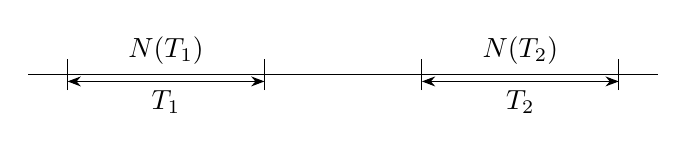
\begin{tikzpicture}
\draw(-4,0)--(4,0)
(1,-0.2)--(1,0.2)
(3.5,-0.2)--(3.5,0.2)
(-1,-0.2)--(-1,0.2)
(-3.5,-0.2)--(-3.5,0.2)
(2.25,0)node[above]{$N(T_2)$}
(-2.25,0)node[above]{$N(T_1)$}
(2.25,-0.08)node[below]{$T_2$}
(-2.25,-0.08)node[below]{$T_1$};
\draw[-Stealth](2.25,-0.09)--(3.5,-0.09);
\draw[-Stealth](2.25,-0.09)--(1,-0.09);
\draw[-Stealth](-2.25,-0.09)--(-3.5,-0.09);
\draw[-Stealth](-2.25,-0.09)--(-1,-0.09);
\end{tikzpicture}
\end{figure}
$N(T_1)$ and $N(T_2)$ are independent random variables.\\

\textit{Stationary Increments:} A counting process is said to have stationary increments if the number of events occurring in time interval $(s, s + t)$  does not depend on $s$ but only on length of interval $(t)$.

\begin{defn}
 A function $f(\cdot)$ is said to be of (order of $h$)  $O(h)$ if $$\lim_{h\rightarrow 0} \frac{f(h)}{h}  = 0.$$
\end{defn}
e.g $f(x)  = x$ (not $O(h)$). $f(x) = x^2$ (of $O(h)$).



\section{Poisson Process}
The counting process $\{N(t),\, t\geq 0\}$ is said to be a Poisson process having rate $\lambda, \hspace{0.2cm} \lambda > 0$ if 
\begin{enumerate}
\item[(i)] $N(0) = 0$
\item[(ii)] $\{N(t)\}$ has independent and stationary increments.
\item[(iii)] $P\left(N(h) = 1\right) = \lambda \, h + O(h)$
\item[(iv)] $P(N(h) > 1) = O(h)$
\end{enumerate}
$$P(N(h) = 0) = 1 - P(N(h) = 1) + P(N(h) \geq 1) = 1 - \lambda\, h.$$

Let $P_n(t) = P(N(t) = n)$
\begin{align*}
P_0(t + \Delta t) & = P(\text{no event in}\, (0,t)\, \text{and}\, \text{no event in}\, (t, t + \Delta t))\\
& = P(N(t + \Delta t) = 0)\\
& = P_0(t) \,(1 - \lambda\,\Delta t).
\end{align*}
As $\Delta t  \longrightarrow 0$, we get
$$\frac{P_0(t  + \Delta t) - P_0(t)}{\Delta t} = -\lambda$$

$$P'_0(t) = -\lambda \, P_0(t)$$
We'll solve this differential equation using the initial condition $P_0(0)  = 1.$
$$\frac{P'_0(t)}{P_0(t)} =- \lambda$$
$$\int\frac{P'_0(t)}{P_0(t)}\, dt =\int(-\lambda)\, dt$$
$$\ln P_0(t) = -\lambda \, t  + C$$
$$P_0(t) = K\, e^{-\lambda t}$$
where $K = e^C$.
$$P_0(0)= K\, e^0  = 1\, \implies\, K  = 1$$

$$\therefore\,\hspace{0.3cm} P_0(t) = e^{-\lambda t}.$$



$$P_1(t + \Delta t) = P_0(t) (\lambda \, \Delta t)  + P_1(t)(1 - \lambda \, \Delta t).$$
As $\, \Delta t  \longrightarrow \, 0$, 
$$P'_1(t) = \lambda\, P_0(t) - \lambda\, P_1(t)$$
$$P'_1(t) = \lambda\, e^{-\lambda t} - \lambda\, P_1(t)$$
$$P_1'(t)  + \lambda \, P_1(t)   = \lambda\, e^{-\lambda t}$$

$$I.F  = e^{\int \lambda \, dt} = e^{\lambda t}$$

$$e^{\lambda t}\, P_1(t)  = \lambda \int e^{\lambda t}\, e^{-\lambda\, t}\, dt + K$$
$$e^{\lambda\, t}\, P_1(t)    = \lambda \, t + K$$
Since $N(0) = 0, \hspace{0.3cm} P_1(0) = 0$, substituting $t = 0$, in the above equation. We get  $ K = 0$. Hence $$P_1(t) = e^{-\lambda t}\, \lambda\, t.$$


Generalizing the above two results 
$$P_n(t) = \frac{e^{-\lambda t}\, (\lambda t)^n}{n!}\hspace{0.2cm} , \hspace{0.5cm} n = 0, \, 1, \, 2, \, \cdots\cdots$$





\section{Interarrival and Waiting Time Distributions}
Consider a Poisson process $\{N(t), \, t\geq 0\}$ of rate $\lambda$.\\

\textit{Interarrival time:} Time between two consecutive arrivals.\\

\textit{Waiting time of the $n^{\text{th}}$ event $W_n$} is the waiting time of the $n^{\text{th}}$ event i.e time from $t = 0$ to the instant when $n^{\text{th}}$  event occurred.

$$P(T_1 > t) = P(N(t) = 0) = e^{-\lambda t}.$$
Hence $P(T_1 \leq t) = 1 - e^{-\lambda t}\,$ (Distribution function of $T_1$) 
$$f_{T_1}(t) = \lambda\, e^{-\lambda t}.$$
Hence $T_1$ follows exponential distribution with parameter $\lambda$.\\


Distribution of $T_2$.
\begin{align*}
P\left(T_2 > t\, |\, T_1 = s\right) & = P\left(N(s, s + t) = 0\, |\, N(s) = 1\right)\\
& =P\left(N(s, s+ t) = 0\right)\\
&  = e^{-\lambda t}.
\end{align*}
Distribution of $T_2$ is also exponential.\\

$\{T_1, \, T_2, \, \cdots\, T_n\}-$ each is an exponential.\\



Let $F_{S_n}(t)$ be the distribution function of random variable $S_n$ (waiting time)
\begin{align*}
F_{S_n}(t) & = P\left(S_n \leq t\right)\\
& = P\left(N(t) \geq n\right)\\
& = \sum^{\infty}_{i = n} \frac{e^{-\lambda\, t}\, (\lambda t)^i}{i!}.
\end{align*}
Density function
$$f_{S_n}(t) = \frac{d}{dt}\, F_{S_n}(t)$$
where $f_{S_n}(t)$ is the pdf of $S_n$
\begin{align*}
f_{S_n}(t) & = \sum^{\infty}_{i = n} \frac{1}{i!} \left(-\lambda\, e^{-\lambda t}\, (\lambda t)^i + i\, \lambda\, (\lambda t)^{i -1}\, e^{-\lambda t}\right)\\
& = -\lambda\, \sum^{\infty}_{i = n} \frac{e^{-\lambda t}\, (\lambda t)^i}{i!} \, + \, \sum^{\infty}_{i = n} \frac{\lambda\, e^{-\lambda t}\, (\lambda t)^{i  - 1}}{(i - 1)!}\\
& =  -\lambda\, e^{-\lambda t}\, \sum^{\infty}_{i = n} \frac{(\lambda t)^i}{i!} + \frac{\lambda\, e^{-\lambda t}\, (\lambda t)^{n - 1}}{(n - 1)!} + \sum^{\infty}_{i = n+ 1} \lambda\, e^{-\lambda t}\, \frac{(\lambda t)^{i  - 1}}{(i - 1)!}\\
& = \frac{\lambda\, e^{-\lambda t}\, (\lambda t)^{n - 1}}{(n - 1)!}\hspace{0.2cm} , \hspace{0.5cm} t >0.
\end{align*}
$S_n$ is Gamma random variable.



\begin{exa}
\begin{enumerate}
\item Suppose that people immigrate into a territory at a Poisson rate $\lambda = 1$ per day.
      \begin{enumerate}
        \item What is the expected time until the tenth immigrant arrives?
        \begin{proof}[\textbf{\textit{Solution.}}]
        $E\left(S_{10}\right) = \dfrac{10}{1} = 10$ days.
        \end{proof}
        
        \item what is  the probability that the elapsed time between the tenth and eleventh arrival exceeds two days?
        \begin{proof}[\textbf{\textit{Solution.}}]
        $\begin{aligned}[t]
        P(T_{11} > 2) &  = \int^{\infty}_2 e^{-x}\, dx \\
        & = \lim_{a\rightarrow \infty} \int^a_2 e^{-x}\, dx\\
        & = \lim_{a\rightarrow \infty} \left[-e^{-x}\right]^a_2\\
        & = \lim_{a\rightarrow \infty} \left[-e^{-a} + e^{-2}\right]\\
        & = e^{-2}.
        \end{aligned}$\\
        \end{proof}
      \end{enumerate}
      
      
\item The time required to repair a machine is an exponential distribution random variable with mean $\frac{1}{2}$ hrs. What is the probability that repair time exceeds $\frac{1}{2}$ hours.

\begin{proof}[\textbf{\textit{Solution.}}]
$\dfrac{1}{\lambda} = \dfrac{1}{2}\, \implies\, \lambda = 2.$
$$Pdf. \, = 2\, e^{-2x}\hspace{0.3cm} , \hspace{0.4cm} x \geq 0$$
\begin{align*}
P\left(X\geq \frac{1}{2}\right) & = \int^{\infty}_{\frac{1}{2}} 2\, e^{-2\,x }\, dx\\
&  = \lim_{k \rightarrow \infty} \int^k_{\frac{1}{2}} 2\, e^{-2\, x}\, dx\\
&  = e^{-1}.
\end{align*}
\end{proof}
\end{enumerate}
\end{exa}



















\section{Further Properties of Poisson Process}
\textbf{\bf 4.4.1.}\,\,  Consider a Poisson process $\{N(t), \, t\geq 0\}$ having rate $\lambda$ and suppose that each time an event occurs, it is classified  as either  a type $I$ or type $II$  event. Suppose further that each event is classified as type $I$ with probability $p$ and as type $II$ event with probability $1 - p$, independently of all other events.\\

Let $N_1(t)$ and $N_2(t)$ be the number of type $I$ and type $II$ events occuring in $[0,t]$.\\


\textit{Proposition.} $\{N_1(t),\, t\geq 0\}$ and $\{N_2(t), \, t\geq 0\}$ are both Poisson process having rates $\lambda p$ and $\lambda (1 - p)$ respectively. Furthermore the two process are independent.

\begin{proof}
Clearly $N(t) = N_1(t) + N_2(t)$. Let $m$ be a non negative integer
\begin{align*}
P(N_1(t) = m) & = \sum^{\infty}_{n =m} P\left(N_1(t) = m\, \big|\, N(t) = n\right)P(N(t) = n)\\
       &  =  \sum^{\infty}_{n = m}\binom{n}{m}\, p^m\, (1 - p)^{n - m}\, \frac{e^{-\lambda t}\, (\lambda t)^n}{n!}\\
       & = p^m\, e^{-\lambda t}\, \sum^{\infty}_{n = m} \frac{n!}{(n - m)!\, m!}\, (1 - p)^{n - m}\, \frac{(\lambda t)^n}{n!}\\
       & = \frac{p^m\, e^{-\lambda t}}{m!}\, \sum^{\infty}_{n =m} \, \frac{(1 - P)^{n - m}}{(n - m)!}\, (\lambda t)^n\\
       & = p^m\, \frac{e^{-\lambda t}}{m!}\, (\lambda t)^m\, \sum^{\infty}_{n = m}\frac{(1 - P)^{n - m}}{(n  - m)!}\, (\lambda t)^{n -m}\\
       & = (p\, \lambda t)^m\, \frac{e^{-\lambda t}}{m!}\, \left(1  + \frac{(1 - p)}{1!}\, \lambda t + \frac{(1 - p)^2\, (\lambda t)^2}{2!} + \cdots\cdots\right)\\
       & = (p\, \lambda t)^m\, \frac{e^{-\lambda t}}{m!}\, e^{(1 - p)\lambda t}\\
       & = \frac{e^{-p\lambda t}\, (p\lambda t)^m}{m!}.
\end{align*}
Hence $N_1(t)$ has a Poisson process of rate $p\lambda$.\\

Similarly $N_2(t)$ has a Poisson process of rate $(1 -  p)\lambda$.
\begin{align*}
P\left(N_1(t) = n_1\, , \,  N_2(t) = n_2\right) &  = P(N_1(t) = n_1\,  ,\, N(t) = n_1 + n_2)\\
 & = P(N_1(t) = n_1\, |\, N(t) = n_1 + n_2)\, P(N(t) = n_1 + n_2)\\
 & = \binom{n_1 + n_2}{n_1}\, p^{n_1}\, (1 - p)^{n_2}\, e^{-\lambda t}\, \frac{(\lambda t)^{n_1 + n_2}}{(n_1 + n_2)!}\\
 & = \frac{(n_1 + n_2)!}{n_1!\, n_2!}\, p^{n_1}\, (1 - p)^{n_2}\, \frac{e^{-\lambda t}\, (\lambda t)^{n_1 + n_2}}{(n_1 + n_2)!}\\
 & = \frac{p^{n_1}\, (1 - p)^{n_2}}{n_1!\, n_2!}\, e^{-\lambda t}\, (\lambda t)^{n_1}\, (\lambda t)^{n_2}\\
 & = \frac{e^{-\lambda t + p\lambda t - p\lambda t}}{n_1!\, n_2!}\, p^{n_1}\, (1 - p)^{n_2}\, (\lambda t)^{n_1}\, (\lambda t)^{n_2}\\
 & = \frac{e^{-\lambda t + p\lambda t - p\lambda t}}{n_1!\, n_2!}\, (p(\lambda t))^{n_1}\, ((1-p)\lambda t)^{n_2}\\
 & = \frac{e^{-p\lambda t} \, (p\lambda t)^{n_1}}{n_1!}\, \cdot\, \frac{e^{-\lambda t(1 - P)}\, ((1 - p)\lambda t)^{n_2}}{n_2!}\\
 & = P(N_1(t) = n_1)\cdot P(N_2(t)  = n_2).
\end{align*}
\end{proof}




















\newpage
\chapter{Birth and Death Process}
\section{The Simple Birth Process}
Let $X(t)$ denote the size of population at time $t$. Let $P_n(t) = P\left(X(t) = n\right).$\\

Assume all individuals in the population are capable of giving birth to new individuals. Let the probability of a given individual producing a new one in time $\Delta t$ be $\lambda \Delta t$ and not producing in time $\Delta t$ be  $1 - \lambda\Delta t$. Assume further that individuals produce independently.\\

Let $P_n(t) = P\left(X(t) = n\right)$
\begin{enumerate}
\item[$*$] $\lambda \Delta t -$ individual produces
\item[$*$] $1 - \lambda \Delta t-$ individual doesn't produce.
\end{enumerate}
\begin{align*}
P_n\left(t + \Delta t\right)  = & P\left(X(t) = n\, \, \text{and no birth in time}\,\, \Delta t\right) + P\left(X(t) = n - 1\,\,\text{and one birth in time}\, \, \Delta t\right)\\
= & P_n(t)\left[\lambda \Delta t (1 - \lambda t)(1 - \lambda \Delta t) \, \cdots\, (1 - \lambda \Delta t)\right] + P_{n - 1}(t)[\lambda \Delta t (1 - \lambda \Delta t)\, \cdots\, (1 - \lambda \Delta t)\\ 
& + (1-\lambda \Delta t)\lambda \Delta t(1 - \lambda \Delta t)\, \cdots\, (1 - \lambda\Delta t) + \cdots + (1 - \lambda \Delta t) \cdots(1 - \lambda \Delta t)(\lambda \Delta t)]\\
& = P_n(t)\left(1 - n\lambda \Delta t\right) + P_{n - 1}(t)(n - 1)\lambda \Delta t.
\end{align*}

$$\frac{P_n(t + \Delta t) - P_n(t)}{\Delta t} = -n\, \lambda \, P_n(t)  + (n - 1)\, \lambda \, P_{n - 1}(t)$$
as $\Delta t \longrightarrow 0$,
$$P'_n(t) = -n\lambda P_n(t)  + (n - 1)\, \lambda\, P_{n - 1}(t).$$

Assume $X(0) = a.$ i.e $P_a(0) = 1$.\\


Let $M(\theta,t)$ denote the mgf of $X(t)$. Then
\begin{align*}
M(\theta,t) & = E\left(e^{\theta\, X(t)}\right)\\ 
&= \sum^{\infty}_{n = 0} e^{\theta n}\, P_n(t)\\
& = P_0(t) + P_1(t)\, e^{\theta} + P_2(t)\, e^{2\theta} + \cdots
\end{align*}
Hence $M(\theta,0) = e^{\theta\, a}$.
$$M(\theta,t) = \sum^{\infty}_{n  = 0} e^{n\theta}\, P_n(t)$$
$$\frac{\partial M}{\partial\theta} = \sum^{\infty}_{n  = 0} n\, e^{n\theta}\, P_n(t)$$
$$\frac{\partial M}{\partial t}  = \sum^{\infty}_{n = 0} e^{n\theta}\, P_n'(t).$$
Now coming back to the equation
$$P'_n(t) = -n\, \lambda \, P_n(t) + (n- 1)\, \lambda \, P_{n - 1}(t)$$
multiply across by $e^{n\theta}$ and sum for $n$ from 0 to $\infty$.
$$\sum^{\infty}_{n = 0} P'_n(t)\, e^{n\theta} \, = \, \sum^{\infty}_{n = 0}-n\, \lambda\, P_n(t)\, e^{n\theta} \, + \, \sum^{\infty}_{n = 0}(n - 1)\, \lambda\, P_{n - 1}(t)\, e^{n\theta}.$$

$$\frac{\partial M}{\partial t} = -\lambda \, \frac{\partial M}{\partial\theta} + \lambda\, \sum^{\infty}_{n = 0}(n -1)\, e^{\theta(n - 1)}\, P_{n -1}(t)\, e^{\theta}.$$

$$\frac{\partial M}{\partial t}  = -\lambda\, \frac{\partial M}{\partial \theta} \,  + \, \lambda\, e^{\theta}\, \frac{\partial M}{\partial \theta}.$$
We'll solve this PDF with the initial condition $M(\theta,0) = e^{a\theta}$.
$$\frac{\partial M}{\partial t} \, +\, \lambda\left(1 - e^{\theta}\right)\, \frac{\partial M}{\partial \theta} = 0.$$

For solving the PDF, we find two independent general solution for the equations
$$\frac{dt}{1} = \frac{d\theta}{\lambda\left(1 - e^{\theta}\right)} = \frac{dM}{0}$$
$$\frac{dt}{1} = \frac{dM}{0}\, \implies\, dM = 0\hspace{0.5cm}\text{i.e}\hspace{0.2cm} M = \text{constant}$$
Find a general solution of 
$$\frac{dt}{1} = \frac{d\theta}{\lambda\left(1 - e^{\theta}\right)}$$

$$\lambda\, dt = \frac{d\theta}{e^{\theta}\, \left(e^{\theta} - 1\right)}$$

$$-\lambda\, dt = \frac{- e^{-\theta}}{e^{-\theta} - 1}\, d\theta$$
$$C - \lambda \, t  = \ln\left(e^{-\theta} - 1\right)$$
$$e^C\, e^{-\lambda\,t} = e^{-\theta} - 1$$
$$e^{\lambda\,t}\, \left(e^{-\theta} - 1\right) = \text{constant}.$$
Hence the general solution of the PDF is 
$$M(\theta,t) = \Phi\left(e^{\lambda t}\, \left(e^{-\theta} - 1 \right)\right)$$

$$M(\theta,0) = \Phi\left(e^{-\theta} - 1\right)$$
but $M(\theta,0)  = e^{a\theta}$. Hence
$$\Phi\left(e^{-\theta} - 1\right) = e^{a\theta}.$$
Let $y = e^{-\theta} - 1$
$$e^{-\theta} = y + 1$$
$$e^{\theta} = \frac{1}{y + 1}$$
$$e^{a\theta} = \left(\frac{1}{y  + 1}\right)^a.$$

Hence the mapping $\Phi$ is 
$$\Phi(y) = \left(\frac{1}{y + 1}\right)^a.$$
Hence
\begin{align*}
M(\theta, t) & = \left(\frac{1}{e^{\lambda t}\left(e^{-\theta} - 1\right) + 1}\right)^a = \left(e^{\lambda t}\, \left(e^{-\theta}  - 1\right) + 1\right)^{-a}
 = \left[1 - e^{\lambda t}\, \left(1 - e^{-\theta}\right)\right]^{-a}.
\end{align*}

Now, the Negative Binomial $-$ Number of failures before the $r^{\text{th}}$ success. We find the MGF of the Negative Binomial
$$P(Y=n) = \binom{n - 1}{r - 1}\, P^{r - 1}\, q^{n - r}\, P\, , \hspace{0.3cm} n\geq r.$$

PGF of $y = E\left(\theta^y\right)$

\begin{align*}
E\left(\theta^y\right) & = \sum^{\infty}_{n = r}\theta^n\, \binom{n - 1}{r - 1}\, p^r\, q^{n - r}\\
& = \left(\frac{p}{q}\right)^r\, \sum^{\infty}_{n = r} \frac{(n - 1)!}{(n - r)!(r - 1)!}\, \left(\theta q\right)^n\\
& = \left(\frac{p}{q}\right)^r\,\left[\left(\theta q\right)^r + r\left(\theta q\right)^{r + 1} + \frac{r(r + 1)}{2!}\, \left(\theta q\right)^{r + 2} + \cdots\cdots\right]\\
& = \left(\frac{p}{q}\right)^r\,\left(\theta q\right)^r\left[1 + r \left(\theta q\right) + \frac{r(r+1)}{2!}\, \left(\theta q\right)^2 + \cdots\cdots\right]\\
& = \left(p\theta\right)^r\, \left[1  + r\, \left(\theta q\right) + \frac{r(r + 1)}{2!}\,\left(\theta q\right)^2 + \cdots\cdots\right]\\
& = \left(p\theta\right)^r\, \left(1 - \theta q\right)^{-r}.
\end{align*}

MGF of negative Binomial distribution is derived from the PGF of the distribution by replacing $t$ with $e^t$.\\
Hence MGF of Neg-distribution is 
\begin{align*}
M(\theta)  & = \left(p\,e^{\theta}\right)^r\, \left(1 - e^{\theta}\, q\right)^{-r} = \left(\frac{1 - e^{\theta}\, q}{p\, e^{\theta}}\right)^{-r}\\
& = \left[\frac{1}{p\, e^{\theta}} - \frac{q}{p}\right]^{-r}\\
& = \left[\frac{1}{p}\, e^{-\theta} - \frac{1 - p}{p}\right]^{-r}\\
&  =\left(p^{-1}\, e^{-\theta} - p^{-1}  + 1\right)^{-r}\\
& = \left(1 - p^{-1}\left(1 - e^{-\theta}\right)\right)^{-r}.
\end{align*}
Therefore
$$M(t,\theta)  = \left(1 - e^{\lambda t}\, \left(1 - e^{-\theta}\right)\right)^{-a}.$$
This is the mgf of Negative Binomial distribution with $ p  = e^{-\lambda t}$ and $r = a$.\\
Hence $X(t)$ is a negative Binomial random variable with
$$Prob\left(X(t) = n\right) = \binom{n - 1}{a - 1}\, e^{-a\lambda t}\, \left(1 - e^{-\lambda t}\right)^{n - a}\, ,\hspace{0.3cm} n\geq a.$$
Stochastic mean
$$E(X(t))  = a\left(e^{\lambda t} - 1\right)$$
$$\sigma^2(t) = ae^{\lambda t}\, \left(e^{\lambda t}  - 1\right)$$








\section{Simple Death Process}
Consider a population of individuals which is subject to random death. Assume probability of any individual dying in time $\Delta t$ is $\mu \Delta t$.\\
Assume individuals dies independently and there are $a$ individuals initially. Let $X(t)$ denote the size of the population at time $t$. Then the chance of one death in interval $\Delta t$ is $\mu \, X(t)\, \Delta t$.\\

Let $P_n(t) = P\left(X(t) = n\right)$
$$P_n(t + \Delta t) = P_n(t)\, \left(1 - n\, \mu \, \Delta t\right) + P_{n + 1}(t)(n+1) \mu \Delta t\, , \hspace{0.3cm} n\leq a$$

$$\frac{P_n(t + \Delta t) - P_n(t)}{\Delta t} = -n\, \mu\, P_n(t) + (n + 1)\, \mu\, P_{n + 1}(t).$$
As $\, \Delta t \longrightarrow 0$, 
\begin{equation}
P'_n(t) = -n \, \mu\, P_n(t) + (n + 1)\, \mu\, P_{n + 1}(t)\, ,\hspace{0.3cm} 0\leq n\leq a.
\end{equation}

Let $M(t,\theta)$ be the mgf of $X(t)$.
$$M(t,\theta) = \sum^a_{n  = 0} e^{n\theta}\, P_n(t)$$

$$\frac{\partial M}{\partial \theta}  = \sum^a_{n = 0} n\, e^{n\theta}\, P_n(t)$$
$$\frac{\partial M}{\partial t} = \sum^a_{n  = 0} e^{n\theta}\, P'_n(t).$$

$$X(0) = a\, \implies\, P_a(0) = 1\, \implies\, M(0,\theta) = e^{a\theta}.$$
Multiply equation (5.1) by $e^{n\theta}$ and sum for $n$ from 0 to $a$
$$\sum^a_{n = 0} e^{n\theta}\, P'_n(t) = -\mu\, \sum^a_{n = 0}n\, e^{n\theta}\, P_n(t) + \mu\, \sum^a_{n = 0} (n + 1)\, e^{n\theta}\, P_{n + 1}(t).$$

$$\frac{\partial M}{\partial t} = -\mu\, \frac{\partial M}{\partial \theta} + \mu\, e^{-\theta}\, \frac{\partial M}{\partial \theta}.$$
$$\frac{\partial M}{\partial t} \, + \, \mu\left(1 - e^{-\theta}\right)\, \frac{\partial M}{\partial \theta} = 0.$$

$$\frac{dt}{1}\, =\, \frac{d\theta}{\mu\left(1 - e^{-\theta}\right)}\, = \, \frac{dM}{0}$$
$dM = 0\, \implies \, M = $constant.

$$\mu\, dt = \frac{e^{\theta}}{e^{\theta} - 1}\, d\theta$$
$$A + \mu t  = \ln\left(e^{\theta} - 1\right)$$
$$e^{\theta} - 1 = e^{A + \mu t}$$
$$e^A = e^{-\mu t}\, \left(e^{\theta}  - 1\right).$$
Hence a general solution of the PDF is 
$$M(t,\theta) = \Psi\left(e^{-\mu t}\, \left(e^{\theta} - 1\right)\right).$$
Since $M(0,\theta) = e^{a\theta}$, we have
$$\Psi\left(e^{\theta} - 1\right) = e^{a\theta}.$$


Let $e^{\theta} -  1 = u$
 $$e^{\theta} =  u + 1$$
 $$e^{a\theta} = \left(u  + 1\right)^a$$
 
$$\Psi(u) = \left(u + 1\right)^a$$
Hence 
$$M(t,\theta) = \left[1 + e^{-\mu t}\, \left(e^{\theta} - 1\right)\right]^a.$$

$$P(t,\theta) = \left(1 + e^{-\mu t}\, \left(\theta - 1\right)\right)^a.$$

$Y:$ a binomial random variable $(n,p)$\\
$P(t):$ probability generating function of $Y$


\begin{align*}
P(t) & = \sum^n_{r = 0} t^r\, Pr(t)   = \sum^n_{r = 0} t^r\, C_r^n\, p^r\, q^{n - r}\\
& =\sum^n_{r = 0} C^n_r\, (tp)^r\, q^{n - r}\\
& = (tp + q)^n\\
& = (1 - P + tp)^n\\
& = (1 + p(t - 1))^n.
\end{align*}
$X(t)$ has Binomial distribution with parameters $a$ and $e^{-\mu t}$. \\
Hence $$E(X(t)) = a\, e^{-\mu t}$$
As $\, t \longrightarrow \infty$, \, \, $E(X(t)) \longrightarrow 0$.
i.e eventually the population will die out.







\section{Simple Birth and Death Process}
Every individual in the population is subject to giving birth or dying
\begin{enumerate}
\item[$\lambda\, \Delta t$:] chance of an individual giving birth in time $\Delta t$.
\end{enumerate}
Hence if $X(t)$ represents population size at time $t$, then chance of a birth in interval $\Delta t$ is $\lambda \, \Delta\, X(t)$.
\begin{enumerate}
\item[$\mu\, \Delta t$]: chance of an individual dying in time $\Delta t$.
\end{enumerate}
Assume independence of events birthing and dying and that  individual give birth or die independent of each other.\\

Let $X(t)$ be the size of the population at time $t$.
Assume $X(0) = a$.\\

Let $P_n(t) = P(X(t) = n)$
\begin{align*}
P_n(t + \Delta t) =  & P_n(t)(1 - n\lambda \Delta t)(1 - n\mu\Delta t) + P_{n+1}(t)\left(1 - \overline{n+1}\, \lambda \Delta t\right)\left(\mu(n +1)\Delta t\right)\\
& + P_{n - 1}(t)\left(\overline{n - 1}\, \lambda \Delta t\right)\left(1 - \overline{n - 1}\, \mu \Delta t\right)\\
= & P_n(t)(1 - n\lambda \Delta t  - n\mu\Delta t) + P_{n + 1}(t)\mu(n + 1)\Delta t + P_{n - 1}(t)(n - 1) \lambda \Delta t.
\end{align*}


As $\Delta t  \longrightarrow 0$, 
$$P'_n(t) = -n(\lambda + \mu)\, P_n(t) + \mu(n + 1)\, P_{n + 1}(t) + \lambda (n - 1) \, P_{n - 1}(t)\, , \hspace{0.3cm} n\leq 1.$$

Let 
$$M(t,\theta) = \sum^{\infty}_{n = 0} e^{n\theta}\, P_n(t).$$

$$\frac{\partial M}{\partial t} = -(\lambda + \mu)\, \frac{\partial M}{\partial \theta}  + \mu\, e^{-\theta}\, \frac{\partial M}{\partial \theta} + \lambda\, e^{\theta}\, \frac{\partial M}{\partial\theta}.$$

Assume $X(0) = a$. Then it can be deduced that
$$M(t,\theta) = \left(\frac{1 + \left(e^{\theta}  - 1\right)\left(1 - \lambda t\right)}{1 - \lambda t \, \left(e^{\theta} - 1\right)}\right)^a$$ where $\lambda  = \mu$ which further gives
$$E(X(t)) = \frac{\partial u}{\partial\theta}\Bigg|_{\theta = 0} = a.$$

When $a = 1$, 
$$P(t, \theta) = \frac{1 + (\theta - 1)(1 - \lambda t)}{1 - \lambda t\, (\theta - 1)}.$$

$$P_n(t) = \frac{\left(\lambda t\right)^{n  - 1}}{\left(1 + \lambda t\right)^{n + 1}}\hspace{0.2cm} , \hspace{0.5cm} a = 1, \hspace{0.2cm} \lambda = \mu.$$






\section{Effects of Immigration}
Consider a simple birth and death process which is subject to random immigrants with immigration rate $v$.\\
Hence, chance of an increase in population by one unite in interval of length $\Delta t$, when the population at time $t$ is $n$, is given by $$\left(n\, \lambda \Delta t  + v\, \Delta t\right)$$
which the chance of a loss of one unit in time $\Delta t$ is still $\mu\, X(t)\, \Delta t$
\begin{align*}
P_n(t + \Delta t)  = & P_n(t) (1 -n\, \lambda\, \Delta t - v\, \Delta t)(1 - n\, \mu\, \Delta t) + P_{n - 1}(t)(\overline{n - 1}\, \lambda\, \Delta t + v\, \Delta t)(1 - \overline{n - 1}\, \mu\, \Delta t)\\
& + P_{n + 1}(t) (1 - \overline{n + 1}\, \lambda\, \Delta t - v\, \Delta t)(\overline{n + 1}\, \mu\, \Delta t)\, , \hspace{0.4cm} n\geq 0
\end{align*}






\section{Queues (Consider a Markov Chain with continuous time)}
Let $$P_{ij} (t)   = P\left(X(t + s) = j\, |\, X(s) = i\right).$$
Can a Queue be regarded as an irreducible chain?\\
\textit{Answer:} Yes!\\
Hence a queue (M.C) possesses a limiting (stationary distribution) and we say that the queue is in statistical equilibrium.\\

If  a Markov chain is irreducible then $P_{ij}(t)$ as $t\longrightarrow \infty$ exists and is independent of $i$.
Hence we can take  $$\lim_{t\rightarrow\infty}P_{ij}(t) = P_j.$$
Also
$$\lim_{t\rightarrow \infty} P_{ij}(t) = \lim_{t\rightarrow\infty}P_j(t)  = P_j$$ or  $$\lim_{t\rightarrow \infty}\frac{d\, P_j(t)}{dt} = 0.$$



\vspace*{10pt}
\textbf{\bf 5.5.2.}\,\, A queue system is defined in terms of 
\begin{enumerate}
\item[(i)] Input process (It can be Poisson or by appointment).
\item[(ii)] the queue discipline (First come First serve, ladies first).
\item[(iii)] Service mechanism.
\end{enumerate}


\vspace*{10pt}
\textbf{\bf 5.5.3}\,\, A queue system with one server and no waiting positions.\\
Assume that  chance of a sequence in $(t, t+\Delta t)$ is $\lambda \, \Delta t  + O(\Delta t)$.  Every customer who finds the server occupied leaves the system immediately. If a server is busy with a customer at time $t$ then the customer will end in $(t, t  + \Delta t)$ with probability $\mu \, \Delta t + O(\Delta t)$.\\

Let $N(t)$ be the length of the queue system at time $t$.
$$N(t) = 0, \hspace{0.3cm} 1.$$
Let $$P_n(t) = P\left(N(t) = n\right)$$
$$P_0(t + \Delta t) = P_0(t) (1 - \lambda\, \Delta t) + P_1(t) (\mu\, \Delta t)(1 - \lambda \, \Delta t)$$
$$P'_0(t) = -\lambda\,  P_0(t) + \mu\, P_1(t).$$
As $t \longrightarrow \infty$

$$0 = -\lambda\, P_0 + \mu\, P_1$$

$$P_1 = \frac{\lambda}{\mu}\, P_0$$
since $\, P_0 + P_1 = 1.$
$$P_0 + \frac{\lambda}{\mu}\, P_0 = 1 \, \implies\, P_0 = \frac{\mu}{\mu + \lambda}\hspace{0.5cm}\text{and}\hspace{0.5cm} P_1 = \frac{\lambda}{\mu + \lambda}.$$

Hence when the queue system reaches statistical equilibrium, the probability distribution of the length of queue system is 
$$P_0 = \frac{\mu}{\lambda + \mu}\hspace{1cm} , \hspace{1cm} P_1 = \frac{\lambda}{\lambda + \mu}.$$

\vspace*{10pt}
\textbf{bf 5.5.4}\,\,  Customers arrive at a two shoe shine stand at rate 10 per hour. The average length of a shoe shine is 6 minutes. There is only one attendant so that one chair is used as a waiting positions. Customers who find both chairs occupied go away.
\begin{enumerate}
\item[i.] Assuming Poisson input and exponential service times find the probability distribution of the queue is statistical equilibrium. \\

$\lambda  = 10 $ per hour, \, $\mu = 10$ per hour, $N(t) = 0, 1, 2$.

$$P_0(t + \Delta t) = P_0(t) (1 - 10\Delta t) + P_1(t) (1 - 10\Delta t)(10\Delta t)$$

$$P_1(t + \Delta t) = P_1(t) (10 \Delta t)(10\Delta t) + P_1(t) (1 - 10\Delta t)(1 - 10\Delta t) + P_2(t)(1 - 10\Delta t)(10\Delta t)$$ $$+ P_0(t) (10\Delta t).$$
As $\, \Delta t \, \longrightarrow 0,$
$$P'_0(t) = -10P_0(t)  + 10 P_1(t)$$
$$P'_1(t) = -10P_1(t) + 10 P_0(t) + 10 P_2(t).$$
As $\, t\longrightarrow \, \infty$
$$-10P_0 + 10 P_1 = 0 \, \implies \, P_0  = P_1.$$
$$-20P_1 + 10 P_0   + 10 P_2 = 0\, \implies\, P_2 = 2P_0 - P_0 = P_0.$$
Since $P_0 + P_1  + P_2 = 1$. We get $3P_0 = 1$. Hence limiting distribution of the queue system is $\left(\frac{1}{3}, \, \frac{1}{3}, \, \frac{1}{3}\right).$
\end{enumerate}




\vspace*{10pt}
\textbf{{\bf 5.5.5} M/M/1 Queue.} $M/M/1$, exponential interarrival time/ exponential service/0ne hour.\\
Suppose that customers arrive at a single server service station in accordance with a Poisson Process of rate $\lambda$. That is time between two consecutive arrival are independent exponential random variables having mean $\frac{1}{\lambda}$.\\
Each customer upon arrival, goes directly into service of the server is free and if not the customer joins the queue. When the customer leaves the system and the next customer in line, if there is any entries services.\\
Suppose that the customer service station rate $\lambda$. That is independent. The successive service times are assumed to be independent exponentially distributed random variables having mean $\frac{1}{\mu}$.\\

$X(t) = $ number of customers in the queue system at time $t$.\\
Let $P_n(t) = P(X(t) = n)$
$$P_0(t + \Delta t) = P_0(t) (1  - \lambda\, \Delta t) + P_1(t) (1 - \lambda \, \Delta t)(\mu\, \Delta t).$$
Let $n\geq 1$
$$P_n(t + \Delta t) = P_n(t)(1 - \lambda\, \Delta t) (1 - \mu\, \Delta t)  + P_{n - 1}(t)(\lambda\, \Delta t)(1 - \mu\, \Delta t) + P_{n+1}(t)(1 - \lambda\, \Delta t)(\mu\, \Delta t).$$
As $\, \Delta t \, \longrightarrow \, 0$, 
$$P'_0(t) = - \lambda\, P_0(t) + \mu\, P_1(t)$$
$$P'_1(t) = -(\lambda \mu)\, P_n(t) + \lambda\, P_{n - 1}(t) + \mu\, P_{n + 1}(t)\, , \hspace{0.3cm} n\geq 1.$$

As $\, t\longrightarrow \infty$,\\
the queue system will enter into limiting distribution implying $$P'_n(t) = 0, \hspace{0.5cm} P_n(t) \longrightarrow P_n.$$
Hence we have 
$$-\lambda \, P_0 + \mu\, P_1 = 0\, \implies\, P_1 = \frac{\lambda}{\mu}\, P_0$$
$$-(\lambda + \mu)\, P_n + \lambda \, P_{n - 1} + \mu\, P_{n + 1}  = 0\,  , \hspace{0.3cm} n\geq 1$$

$$\mu\, P_{n + 1} = (\lambda + \mu)\, P_n - \lambda \, P_{n  - 1}\, , \hspace{0.3cm} n\geq 1$$
when $n = 1$, 
\begin{align*}
P_2 & =  \frac{\lambda + \mu}{\mu}\, P_1 - \frac{\lambda}{\mu}\, P_0\\
& = \frac{\lambda + \mu}{\mu}\cdot\left(\frac{\lambda}{\mu}\right)\, P_0 - \frac{\lambda}{\mu}\, P_0\\
& = \frac{\lambda}{\mu}\left(\frac{\lambda + \mu}{\mu} - 1\right)\, P_0\\
& = \frac{\lambda}{\mu}\, \left(\frac{\lambda}{\mu}\right)\, P_0\\
& = \left(\frac{\lambda}{\mu}\right)^2\, P_0
\end{align*}
generalizing $$P_n = \left(\frac{\lambda}{\mu}\right)^n\, P_0.$$
But $P_0 + P_1 + P_2 + \cdots\, = 1$. Hence 
$$P_0 + \frac{\lambda}{\mu}\, P_0 + \left(\frac{\lambda}{\mu}\right)^2 \, P_0 + \cdots\,  = 1$$
i.e
$$\left(1 + \frac{\lambda}{\mu} + \left(\frac{\lambda}{\mu}\right)^2  + \cdots\cdots \right)\, P_0 = 1$$
$$\left(\frac{1}{1 - \dfrac{\lambda}{\mu}}\right)\, P_0 = 1\hspace{0.5cm} \text{provided}\hspace{0.3cm} 0 < \frac{\lambda}{\mu} < 1$$
\begin{align*}
P_0  & = \frac{\mu - \lambda}{\mu}\\\\
P_1 & = \left(\frac{\lambda}{\mu}\right)\, \left(\frac{\mu - \lambda}{\mu}\right)\\\\
P_2 & = \left(\frac{\lambda}{\mu}\right)^2\, \left(\frac{\mu - \lambda}{\mu}\right)\\
   \vdots & 
\end{align*}
where $0 < \frac{\lambda}{\mu} < 1$.\\

Expected number of customers in the queue system in long run $$ = \sum^{\infty}_{n  = 0} n\, P_n.$$




\textbf{\textit{Example.}} Consider a server in which probability that exactly one customer arrive in time $\Delta t$ is $\lambda\, \Delta t$.\\
If there are $j$ customers in service at time $t$, the probability that exactly one customer will complete service in  time $(t , t  + \Delta t)$ is $j\, \mu\, \Delta t$.
$$P_0(t + \Delta t) = P_0(t) (1 - \lambda\, \Delta t) + P_1(t) (1 - \lambda\, \Delta t)(\mu\, \Delta t).$$
Let $n\geq 1$
\begin{align*}
P_n(t + \Delta t)  =  & P_n(t) (1 - \lambda\, \Delta t)(1 - n\, \mu\, \Delta t) + P_{n -1}(t)(\lambda\, \Delta t)(1 - \overline{n - 1}\, \mu \, \Delta t)\\
                      & + P_{n + 1}(t) (1 - \lambda \, \Delta t)(\overline{n  + 1}\, \mu\, \Delta t).
\end{align*}

$$P_j = \frac{\left(\frac{\lambda}{\mu}\right)^j\, e^{-\frac{\lambda}{\mu}}}{j!}\hspace{0.3cm} , \hspace{0.5cm} j = 0, \, 1, \, \cdots\cdots$$























\newpage
\chapter{Brownian Motion}
Consider a stochastic process $\left\{X(t), \, t\geq 0\right\}$ whose state space is an interval of real line such a  process has stationary increments in distribution of $X\left(t + s\right) - X(t)$ does not depend on $t$. This process has independent increments if for $0 < t_1 < t_2 < \cdots < t_n$ the random variables
$$X(t_n) - X(t_{n - 1}),\, X(t_{n - 1}) - X(t_{n - 2}), \, \cdots\, , X(t_2) - X(t_1), \, X(t_1) - X(0)$$ are independent.\\

A stochastic process $\left\{X(t),\, t\geq 0\right\}$ with a real state space is called Brownian motion if the following are true:
\begin{enumerate}
\item[(i)] $X(0) = 0$
\item[(ii)] the process has stationary and independent increments
\item[(iii)] for every $t>0, \, X(t)$ has a normal distribution with mean zero and variance $t\sigma^2$.
\end{enumerate}



If $\sigma^2 =1$, the Brownian motion is called standard Brownian motion.\\

Consider a standard Brownian motion $\left\{X(t), \, \geq 0\right\}$. Let $0 < t_1 < t_2 < \, \cdots\, < t_n$. The set of equations
$$X(t_n) = x_n, \, \, X(t_{n - 1}) = x_{n - 1}, \, \cdots\, \, , \, X(t_1) = x_1$$ is equivalent to 
\begin{align*}
X(t_n)   - X(t_{n - 1}) &  = x_n - x_{n - 1}\\
X(t_{n - 1}) - X(t_{n - 2}) &  = x_{n  - 1} - x_{n - 2}\\
\vdots & \\
X(t_2) - X(t_1) &= x_2, - x_1\\
X(t_1) &  = x_1
\end{align*}
where random variables
$$X(t_n) - X(t_{n - 1}), \, \cdots\, , \, X(t_1)$$
are independent and satisfy the condition of  stationarity.\\

Hence the pdf of $X(t)$ is 
$$f_t(x) = \frac{1}{\sqrt{2\pi t}}\, e^{-\frac{x^2}{2t}}$$
and the distribution of $X(t_i) - X(t_{i -1})$ is normal with mean 0 and variance $(t_i - t_{i -1})$ \textit{(the variance is the length of the interval.)}\\

The joint density of $X(t_1), \, X(t_2), \, \cdots\,  ,\, X(t_n)$ is equal to the joint density of $$X(t_n) - X(t_{n - 1}), \, \cdots\, , \, X(t_1).$$
Hence $f(x_1, \, \cdots\, ,\, x_n) = f_{t_1}(x_1)\, f_{t_2-t_1}(x_2 - x_1)\, \cdots\, f_{t_n - t_{n -1}}(x_n - x_{n - 1}).$\\\\



Let $s < t$.\\
Finding conditional distribution of $X(s)$ given $X(t) = B$
\begin{align*}
f_{s/t}(x,B) & = \frac{f_{s,t}(x, B)}{f_t(B)} = \frac{f_s(x)\, f_{t-s}(B - x)}{f_t(B)}\\\\
&  = \frac{\frac{1}{\sqrt{2\pi s}}e^{-\frac{x^2}{2s}}\, \cdot\, \frac{1}{\sqrt{2\pi(t - s)}}e^{-\frac{(B - x)^2}{2(t - s)}}}{f_t(B)}\\\\
& = K\, \exp\left[\frac{x^2}{2s} - \frac{(B - x)^2}{2(t - s)}\right]\\\\
& = K_1\, \exp\left[\frac{-\left(x - \dfrac{Bs}{t}\right)}{\dfrac{2s(t-s)}{t}}\right].
\end{align*}

For $s <t $
$$E\left(X(s)| X(t) = B\right) = \frac{Bs}{t}$$

$$var\left(X(s)\, |\, X(t)  = B\right) = \frac{s(t - s)}{t}$$




\begin{exa}
In a  bicycle race between two competitors. Let $Y(t)$ denote the amount of time (in seconds) by which the racer that started in the inside position is ahead when $100t\%$ of the race has been completed and suppose that $\left\{Y(t), \, 0\leq t\leq 1\right\}$ can be effectively modeled as a Brownian process with variance $\sigma^2$.\\

\textit{Question (i).} If the inside racer is leading by $\sigma$ seconds at the mid point of the race, what is the probability that she is the winner.
\begin{align*}
P\left(Y(1) > 0\, |\, Y\left(\frac{1}{2}\right) = \sigma\right) = & P\left(Y(1)  -Y\left(\frac{1}{2}\right) > - \sigma \, \Big|\, Y\left(\frac{1}{2}\right) = \sigma\right)\\
  = & P\left(Y(1) - Y\left(\frac{1}{2}\right) > - \sigma\right)\hspace{0.5cm}\text{using conditionalof independent }\\
  & \text{increments}\, X(1) - X\left(\frac{1}{2}\right) \hspace{0.2cm}\text{and}\hspace{0.2cm} X\left(\frac{1}{2}\right)\hspace{0.3cm}\text{independent.}\\
   = & P\left(Y\left(\frac{1}{2}\right) > - \sigma\right)\hspace{0.5cm}\text{stationary increments.}\\
     & Y(t)\, \thicksim\, N(0,t\sigma^2)\hspace{0.3cm}\text{and}\hspace{0.3cmf}  Y\left(\frac{1}{2}\right) \, \thicksim \, N\left(0, \sigma^2\, \frac{1}{2}\right)\\
     & = P\left(\frac{Y\left(\frac{1}{2}\right) - 0}{\sigma\, \frac{1}{\sqrt{2}}}\, > \, \frac{-\sigma - 0}{\sigma\, \frac{1}{\sqrt{2}}}\right)
\end{align*}
$$P(Z > -\sqrt{2}) = 0.9213.$$

\textit{Question (ii).}  If the inside racer wins the race by a margin of $\sigma$ seconds, what is the probability that she was ahead at the mid point.
$$P\left(Y\left(\frac{1}{2}\right) > 0\, \Big|\, Y(1) = \sigma\right)$$
$Y(t)$ is not a standard Brownian motion hence we standardize it as follows:\\

Let $X(t) = \frac{Y(t)}{\sigma}.$
\begin{align*}
P\left(Y\left(\frac{1}{2}\right)  > 0\, \Big|\, Y(1) = \sigma\right) & = P\left(\sigma \, X\left(\frac{1}{2}\right) > 0 \, \Big|\, \sigma\, X(1) = \sigma\right)\\
& = P\left(X\left(\frac{1}{2}\right) > 0\, \Big|\, X(1) = 1\right)
\end{align*}
distribution of $X\left(\frac{1}{2}\right)|X(1) = 1$ is normal with mean $\frac{1/2}{1}\times 1 = \frac{1}{2}$ and variance $= \frac{1/2(1 - 1/2)}{1} = \frac{1}{4}$.
\begin{align*}
& = \left(Z > \frac{0 - 1/2}{1/2}\right) 
 =P(Z > - 1)
 =0.8413.
\end{align*}
\end{exa}






\newpage

\begin{enumerate}
\item[A.] \textbf{Rationale and Objects}\\
This course links the probability theory to its applications in the physical and social sciences and in operations research.\\

At the end of the course, students will have understood and be able to use Markov chains, Poisson processes, continuous-time Markov chains, renewal theory, queuing theory, reliability theory, Brownian motion and stationary processes.


\item[B.] \textbf{Topic Outline}\\
Markov Chain: Markov chains having two states, transition functions and initial distribution, transient and recurrent states, decomposition of state space (absorption probabilities and Martingales), birth and death chains. Stationary distributions of  a Markov chain: elementary properties of stationary distributions, average number of visits to recurrent state, null recurrent and positive recurrent states, queuing chain, convergence to the stationary distribution. Markov pure jump processes: construction of jump processes, birth and death processes, properties of a Markov pure jump process. Second order processes: mean and covariance functions, Gaussian processes, Wiener processes. Continuity, integration and differentiation of second order processes: continuity assumptions, integration, differentiation, white noise.\\


\item[C.]\textbf{Text}
\begin{thebibliography}{}
\bibitem{PGH}{}
Introduction to Stochastic Processes by P G Hoel, S C Port and C J Stone, Houghton Mifflin Co (1972)
\bibitem{IPM}{}
Introduction to Probability Models by Sheldon M. Ross, 5th ed, Academic Press, Inc.(1993)
\end{thebibliography}
\end{enumerate}


\pagebreak


\section{Practice Problems}

\begin{problem}
A Markov chain on $\{1,2\}$ has transition matrix
$$P = \begin{pmatrix} 0.7 & 0.3\\ 0.4 & 0.6 \end{pmatrix}.$$
Find $P^{(2)}$, and find the stationary distribution.
\end{problem}
\begin{solution}
By Chapman--Kolmogorov, $P^{(2)} = P^{2}$:
$$P^{2} = \begin{pmatrix} 0.7(0.7)+0.3(0.4) & 0.7(0.3)+0.3(0.6)\\
0.4(0.7)+0.6(0.4) & 0.4(0.3)+0.6(0.6)\end{pmatrix}
= \begin{pmatrix} 0.61 & 0.39\\ 0.52 & 0.48\end{pmatrix},$$
and each row still sums to one, which is the check.

For the stationary distribution solve $\pi P = \pi$ with $\pi_1+\pi_2=1$:
$$0.7\pi_1 + 0.4\pi_2 = \pi_1 \implies 0.4\pi_2 = 0.3\pi_1
\implies \pi_2 = \tfrac34\pi_1 .$$
With $\pi_1+\pi_2=1$ this gives
$$\pi = \left(\tfrac47,\ \tfrac37\right) \approx (0.571,\ 0.429).$$
The rows of $P^{2}$ are already closer to $\pi$ than those of $P$, which is the
convergence the chain is heading towards.
\end{solution}

\begin{problem}
Show that the simple symmetric random walk on $\mathbb{Z}$ is recurrent, using
the criterion that state $0$ is recurrent when $\sum_n p_{00}^{(n)}$ diverges.
\end{problem}
\begin{solution}
Return to the origin is possible only after an even number of steps, and it
requires equal numbers of left and right moves:
$$p_{00}^{(2n)} = \binom{2n}{n}\left(\tfrac12\right)^{2n},
\qquad p_{00}^{(2n+1)} = 0 .$$
By Stirling's approximation $\binom{2n}{n} \sim 4^{n}/\sqrt{\pi n}$, so
$$p_{00}^{(2n)} \sim \frac{1}{\sqrt{\pi n}} .$$
Hence $\sum_n p_{00}^{(n)}$ behaves like $\sum_n n^{-1/2}$, which diverges. The
origin is recurrent, and since the walk is irreducible every state is.

The exponent is what decides it. In three dimensions the corresponding
probability decays like $n^{-3/2}$, whose sum converges, so the walk is
transient --- the walk returns in one and two dimensions and escapes in three.
\end{solution}

\begin{problem}
A branching process has offspring distribution $P(X=0)=\tfrac14$,
$P(X=1)=\tfrac14$, $P(X=2)=\tfrac12$. Find the probability of eventual
extinction starting from one individual.
\end{problem}
\begin{solution}
The offspring generating function is
$$G(s) = \tfrac14 + \tfrac14 s + \tfrac12 s^{2},$$
and the mean offspring number is $G'(1) = \tfrac14 + 1 = \tfrac54 > 1$, so
extinction is not certain and the extinction probability is the smallest root of
$G(s)=s$ in $[0,1]$.
$$\tfrac12 s^{2} - \tfrac34 s + \tfrac14 = 0
\quad\Longrightarrow\quad 2s^{2} - 3s + 1 = 0
\quad\Longrightarrow\quad (2s-1)(s-1) = 0 .$$
The roots are $s=\tfrac12$ and $s=1$, so the extinction probability is
$$q = \tfrac12 .$$

The two roots are the two possibilities, and which one is taken is decided by
the mean: with $\mu\leq1$ the only root in $[0,1)$ disappears and extinction is
certain, while with $\mu>1$ the smaller root is the answer. Here a population
growing on average by a quarter each generation still dies out half the time.
\end{solution}

\begin{problem}
Customers arrive at a counter as a Poisson process of rate $\lambda = 3$ per
hour. Find the probability that exactly two arrive in a given hour, and the
expected waiting time until the first arrival.
\end{problem}
\begin{solution}
The number in an interval of length $t$ is POI$(\lambda t)$, so with $t=1$,
$$P(N_1 = 2) = \frac{e^{-3}3^{2}}{2!} = \frac{9e^{-3}}{2} \approx 0.224 .$$
The waiting time to the first arrival is exponential with rate $\lambda$, so
$$E(T_1) = \frac{1}{\lambda} = \frac13 \text{ hour} = 20 \text{ minutes}.$$

Worth noting: the expected time to the \emph{next} arrival is $20$ minutes
however long one has already waited, by the memorylessness of the exponential.
That is the property which makes the Poisson process the only counting process
with independent stationary increments.
\end{solution}


\end{document}